\documentclass[9pt]{beamer}

\usepackage{appendixnumberbeamer}
\usepackage{booktabs}
\usepackage[scale=2]{ccicons}
\usepackage{pgfplots}
\usepackage{tikz}
\usepackage{graphics}

\usepgfplotslibrary{dateplot}
\pdfstringdefDisableCommands{\def\translate#1{#1}}
\geometry{paperwidth=140mm, paperheight=105mm}
\usetheme{metropolis}
\bibliographystyle{abbrv}
\setbeamertemplate{frame footer}{Lab - Mechatronics}

\usetikzlibrary{shapes, arrows}
\tikzstyle{startstop} = [rectangle, rounded corners, minimum width=2cm, minimum height=1cm, text centered, draw=black, fill=red!30]
\tikzstyle{io} = [trapezium, trapezium stretches=true, trapezium left angle=70, trapezium right angle=110, minimum width=2cm, minimum height=1cm, text centered, draw=black, fill=blue!30]
\tikzstyle{process} = [rectangle, minimum width=2cm, minimum height=1cm, text centered, text width=2cm, draw=black, fill=orange!30]
\tikzstyle{decision} = [diamond, minimum width=2cm, minimum height=1cm, text centered, draw=black, fill=green!30]
\tikzstyle{arrow} = [thick,->,>=stealth]

\title{Modelling and control of a Magnetic Levitation System}
% \subtitle{Mid-project presentation}
% \date{\today}
\date{December 19, 2024}
\author{Tommaso Bocchietti 10740309 \\ Daniele Cianca 10764733 \\ Sara Orazzo 10995845}
\institute{Politecnico di Milano}
\titlegraphic{\hfill
\includegraphics[height=1.5cm]{pdf/Polimi_logo_header.pdf}}

\begin{document}

\maketitle

\begin{frame}{Agenda}

    \begin{columns}[c, onlytextwidth]

        \begin{column}{0.4\textwidth}

            \setbeamertemplate{section in toc}[sections numbered]
            \tableofcontents

        \end{column}

        \begin{column}{0.6\textwidth}

            \begin{figure}[H]
                \centering
                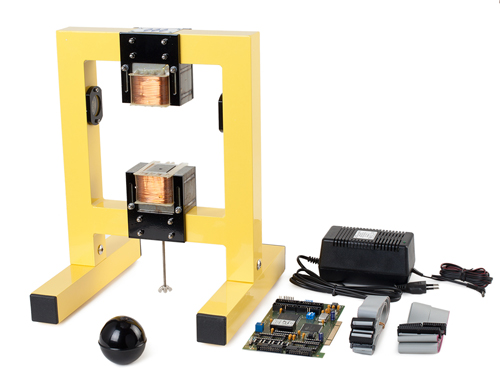
\includegraphics[width=0.8\textwidth]{img/maglev_and_components.jpg}
                \caption{Magnetic Levitation System and its components}
            \end{figure}

        \end{column}

    \end{columns}

\end{frame}

\begin{frame}{Project objectives}

    Magnetic Levitation System (MLS) it's an electromechanical system that enhances magnetic fields to levitate a ferromagnetic object.
    It's known for its non-linear behavior and its instability.

    \begin{columns}[c, onlytextwidth]

        \begin{column}{0.5\textwidth}

            \begin{figure}[H]
                \centering
                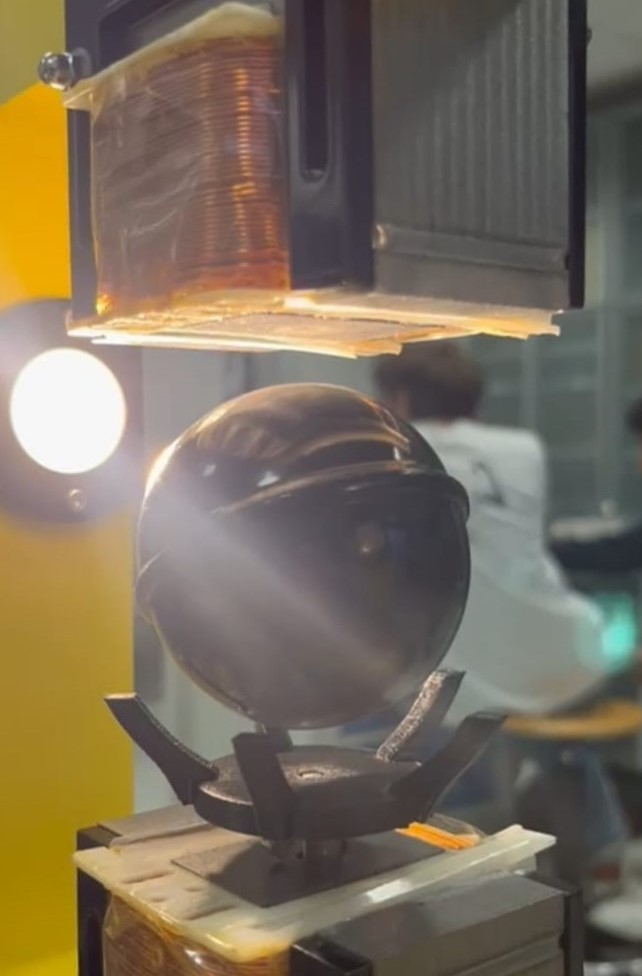
\includegraphics[width=0.7\textwidth]{img/ball_levitation.jpg}
            \end{figure}

        \end{column}

        \begin{column}{0.5\textwidth}

            \begin{center}
                Project objectives: \\
                \textbf{Make the ball levitate.}
            \end{center}

        \end{column}

    \end{columns}



\end{frame}
\begin{frame}{Introduction}

    \hl{Do we want to explain the MagLev?}

    Composed of:

    \begin{itemize}
        \item The ball
        \item The electromagnet
        \item The controll unit (Arduino)
    \end{itemize}

    Etc..

\end{frame}
\section{Modelling}

\begin{frame}{Scheme of MLS system}

    Even if MLS is composed of two coils, for the aim of this work we have chosen to focus on the \textbf{single coil configuration}, considering only the upper one.

    \begin{figure}[H]

        \begin{minipage}{0.40\textwidth}

            \centering

            \begin{tikzpicture}[european voltages]

                \def\radius{0.3}

                % Upper circuit
                \draw (-3, 3.5) node [right] {$+$}
                to [short] ++(0, -1)
                to [R, l^=$R$, resistors/zigs=6] ++(2, 0)
                to [variable cute inductor, i>^=$\dot{q}$, l=$L$] ++(2, 0)
                to [short] ++(0, +1) node [right] {$-$};

                % Reference system
                \draw[|->] (-1.0, +2.5) -- ++(0, -2.5 + \radius) node[left] {$z$, $\dot{z}$, $\ddot{z}$};

                % Ball
                \filldraw[fill=gray, draw=black] (0, 0) circle (\radius);

                % Upward forces
                \draw[thick, ->] (-0.1, +\radius) -- ++(0, +1.5) node[right] {$F_{\text{em}}$};
                \draw[thick, ->] (+0.0, +\radius) -- ++(0, +1.0) node[right] {$F_{\text{in}}$};
                \draw[thick, ->] (+0.1, +\radius) -- ++(0, +0.5) node[right] {$F_{\text{d}}$};

                % Downward forces
                \draw[thick, ->] (+0.0, -\radius) -- ++(0, -0.5) node[right] {$F_{\text{g}}$};

            \end{tikzpicture}

        \end{minipage}
        %
        \hfill
        %
        \begin{minipage}{0.55\textwidth}

            \begin{table}
                \centering

                \begin{tabular}{|c|l|}
                    \hline
                    \textbf{Name}   & \textbf{Description}  \\
                    \hline
                    $F_{\text{g}}$  & Gravitational force   \\
                    $F_{\text{in}}$ & Inertial force        \\
                    $F_{\text{d}}$  & Drag force            \\
                    $F_{\text{em}}$ & Electromagnetic force \\
                    \hline
                \end{tabular}

            \end{table}

        \end{minipage}

        \label{fig:MLS_scheme}

    \end{figure}

\end{frame}



\begin{frame}{Lagrange equation}

    To derive the \textbf{equations of motion}, we started from the Lagrange equation of the system:

    \begin{equation}
        \frac{d}{dt} \left( \frac{\partial \mathcal{T}}{\partial \dot{\mathbf{u}}} \right) - \frac{\partial \mathcal{T}}{\partial \mathbf{u}} + \frac{\partial \mathcal{D}}{\partial \dot{\mathbf{u}}} + \frac{\partial \mathcal{U}}{\partial \mathbf{u}} = \mathcal{Q}
        \text{, where }
        \mathbf{u} = \begin{bmatrix} z \\ q \end{bmatrix}
        \label{eq:lagrange_equation}
    \end{equation}

    The energy terms are defined as follows:

    \begin{equation}
        \begin{aligned}
            \mathcal{T} & = \frac{1}{2} m \dot{z}^2 + \frac{1}{2} L(z, \dot{q}) \dot{q}^2                                                       \\
            \mathcal{D} & = \int_{\dot{z}(\cdot)} \frac{1}{2} C_d A \rho \dot{z}^2 d\dot{z} + \int_{\dot{q}(\cdot)} R(\dot{q}) \dot{q} d\dot{q} \\
            \mathcal{U} & = -m g z - q V                                                                                                        \\
            \mathcal{Q} & = 0
        \end{aligned}
    \end{equation}

\end{frame}



\begin{frame}{Electrical components model}

    Based on experimental data, we have proposed a model for both the resistance and the coil inductance:

    \begin{equation}
        \begin{aligned}
            R & = R(I) = R_{0}                                                          \\
            L & = L(z, I) = L_{0} + L_{z} e^{-a_{z} z} + L_{I} \arctan(a_{I} I - b_{I})
        \end{aligned}
        \label{eq:model_for_inductance}
    \end{equation}

    The first and second derivatives with respect to ball position and current are:

    \begin{equation}
        \begin{aligned}
            \frac{\partial L}{\partial z}     & = -a_{z} L_{z} e^{-a_{z} z}  \\
            \frac{\partial^2 L}{\partial z^2} & = a_{z}^2 L_{z} e^{-a_{z} z}
        \end{aligned}
        \qquad
        \begin{aligned}
            \frac{\partial L}{\partial I}     & = \frac{L_{I} a_{I}}{1 + (a_{I} I - b_{I})^2}                            \\
            \frac{\partial^2 L}{\partial I^2} & = -2 \frac{L_{I} a_{I}^2 (a_{I} I - b_{I})}{(1 + (a_{I} I - b_{I})^2)^2}
        \end{aligned}
        \label{eq:model_for_inductance_derivatives}
    \end{equation}

\end{frame}



\begin{frame}{Model approximations}

    In order to simplify the model, some approximations have been considered:

    \begin{equation}
        \begin{cases}
            \frac{\partial L}{\partial I}     & \approx 0 \\
            \frac{\partial^2 L}{\partial I^2} & \approx 0 \\
            \dot{z}                           & \approx 0
        \end{cases}
        \label{eq:model_reduction_conditions}
    \end{equation}

    Notice that, from successive analysis, these approximations have proven (at least in the range of interest) to be valid.

\end{frame}



\begin{frame}{Equations of motion}

    By applying approximations of Equation (\ref{eq:model_reduction_conditions}) to the Lagrange equation (\ref{eq:lagrange_equation}), we have obtained the following equations of motion:

    \begin{equation}
        \begin{cases}
            \dot{z} = v                                                                         \\
            \dot{v} = m^{-1} \left(\frac{1}{2} \frac{\partial L}{\partial z} I^2 + m g  \right) \\
            \dot{I} = L^{-1} \left(- R I + V \right)
        \end{cases}
        \label{eq:equations_of_motion_single_coil}
    \end{equation}

    Model non-linearities are hidden in all the terms relative to the inductance $L$ and its derivatives.

    \vspace{9pt}

    Despite the applied approximations, the set of Equations (\ref{eq:equations_of_motion_single_coil}) is still \textbf{able to capture the main dynamics of the system}.

\end{frame}

\section{Parameters identification}

\begin{frame}{Overview of the performed tests}

    In order to control the system, we had to \textbf{identify the parameters of the system}.
    To do so, many experiments have been conducted:

    \begin{enumerate}
        \item \textbf{Direct measurement};
        \item \textbf{Sensor characterization};
        \item \textbf{Control-to-voltage dependency};
        \item \textbf{Inductance characterization};
        \item \textbf{Force validation}.
    \end{enumerate}

\end{frame}



\begin{frame}{Direct measurement}

    Many of the parameters of the system can be directly measured using a scale, a caliper or a voltmeter.

    \begin{table}[H]

        \centering
        \begin{tabular}{|c|c|c|}
            \hline
            \textbf{Parameter} & \textbf{Value} & \textbf{Units} \\
            \hline
            $g$                & $9.81$         & $m/s^2$        \\
            $m$                & $0.06157$      & $kg$           \\
            $r$                & $0.06125/2$    & $m$            \\
            $h$                & $0.098$        & $m$            \\
            $R_{0}$            & $4.17$         & $\Omega$       \\
            \hline
        \end{tabular}

        \caption{Directly measured parameters and constants}
        \label{tab:directly_measured_parameters}

    \end{table}

\end{frame}



\begin{frame}{Sensor characterization}

    \only<1>{

        Voltage to position mapping.

        \begin{figure}[H]
            \centering
            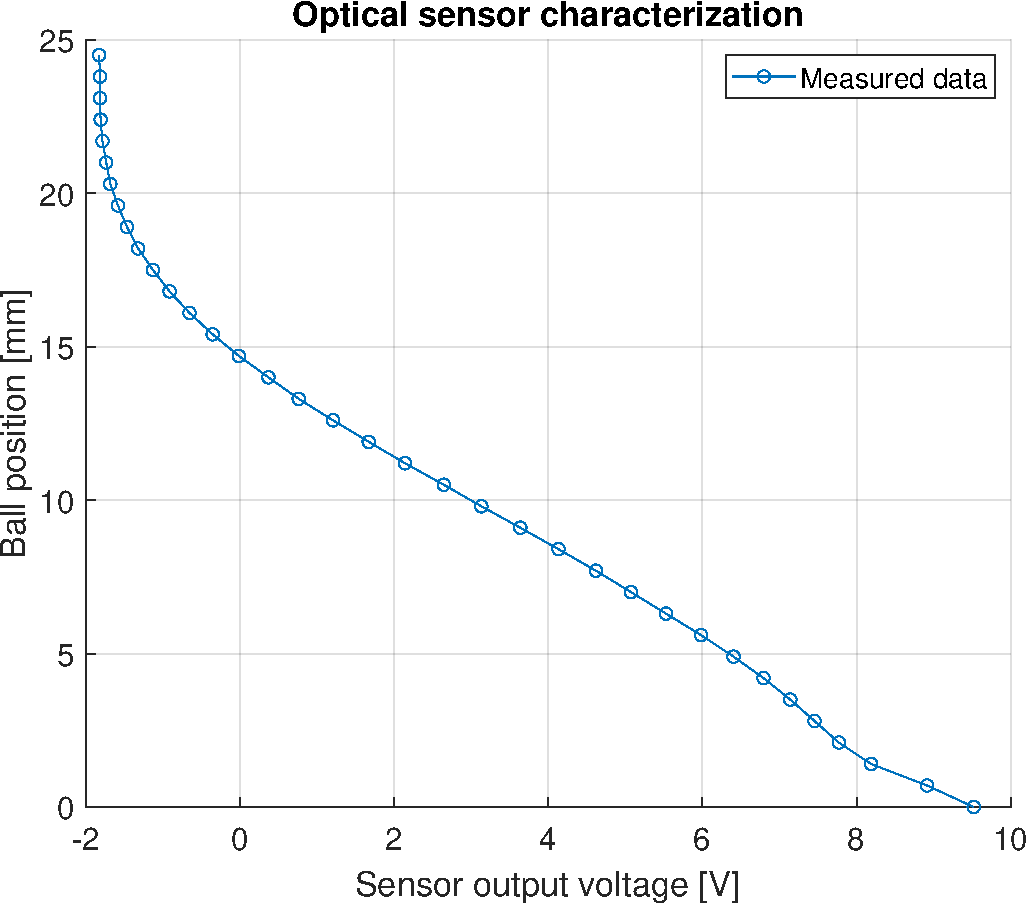
\includegraphics[width=0.6\textwidth]{img/MATLAB/identification/sensor_position.pdf}
            \caption{Position of the ball as a function of the output voltage of the infrared optical sensor.}
            \label{fig:voltage_to_position}
        \end{figure}

    }

    \only<2>{

        Sensors noise analysis.

        \begin{figure}[H]
            \centering
            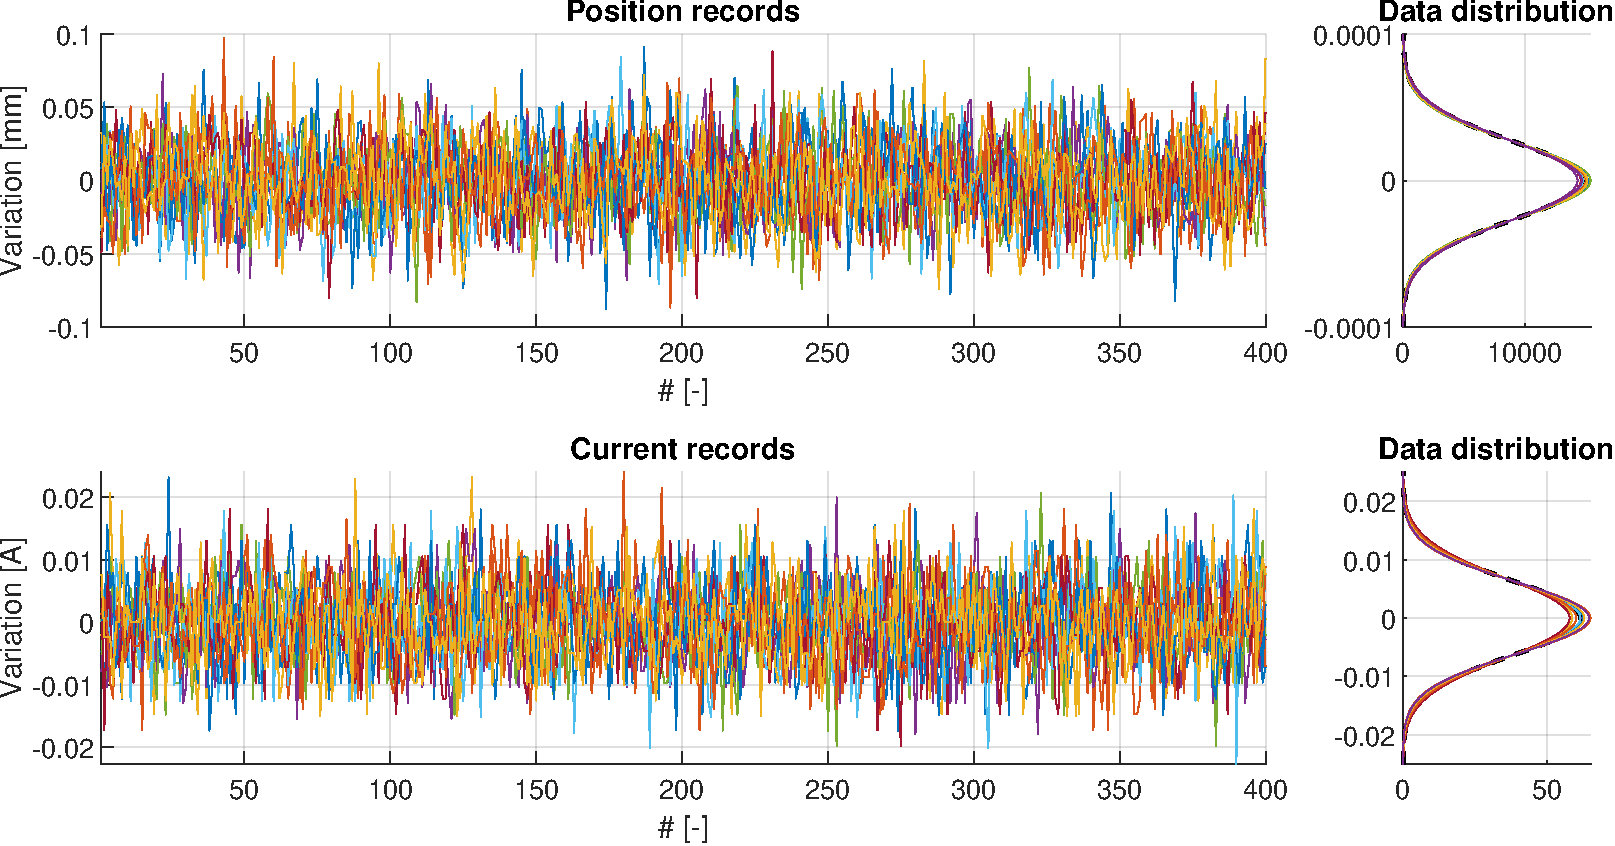
\includegraphics[width=1\textwidth]{img/MATLAB/identification/sensor_noises.pdf}
            \caption{Sensors' noise analysis.}
            \label{fig:sensors_noise}
        \end{figure}

        \begin{table}[H]
            \centering

            \begin{tabular}{|c|c|c|}
                \hline
                \textbf{Sensor} & \textbf{Standard deviation}        & \textbf{Covariance}                  \\
                \hline
                Infrared        & $1.402804 \cdot 10^{-3} \quad [m]$ & $7.166031 \cdot 10^{-6} \quad [m^2]$ \\
                Current         & $6.327979 \cdot 10^{-3} \quad [A]$ & $4.005490 \cdot 10^{-5} \quad [A^2]$ \\
                \hline
            \end{tabular}

            \caption{Standard deviation and covariance of the sensors' noise.}
            \label{tab:sensors_noise}

        \end{table}

    }


    \only<3>{
        Control to Voltage mapping.

        \begin{columns}[c, onlytextwidth]

            \begin{column}{0.45\textwidth}

                As predictable, the control to voltage mapping is a linear function outside the `no control zone'.

                \begin{equation}
                    V = \begin{cases}
                        V_{min} & \text{if } U < U_{min}    \\
                        k U + c & \text{if } U \geq U_{min}
                    \end{cases}
                \end{equation}

            \end{column}

            \begin{column}{0.55\textwidth}

                \begin{figure}
                    \centering
                    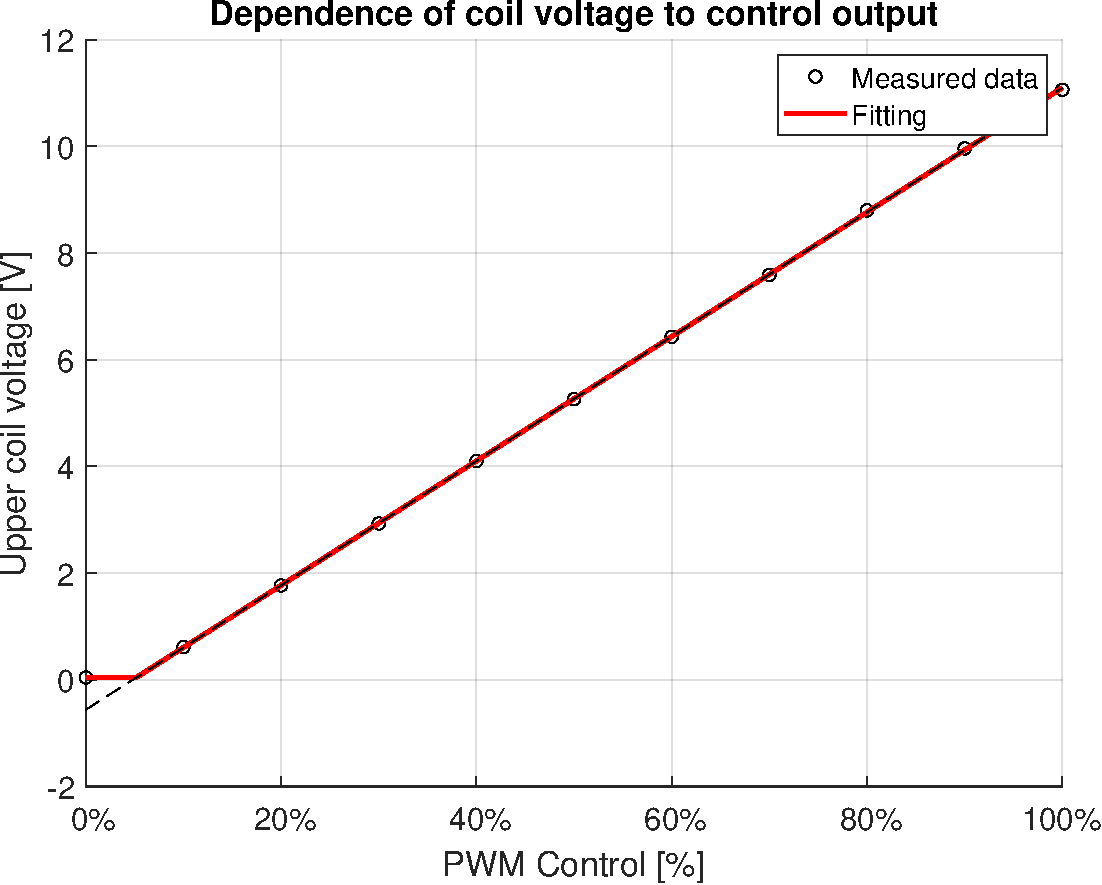
\includegraphics[width=0.8\textwidth]{img/MATLAB/identification/control_to_voltage.pdf}
                    \caption{Voltage as a function of $U$}
                \end{figure}

            \end{column}

        \end{columns}

    }

    \only<3>{
        Electromagnetic force characterizations.

        \begin{columns}[c, onlytextwidth]

            \begin{column}{0.65\textwidth}

                \begin{figure}
                    \centering
                    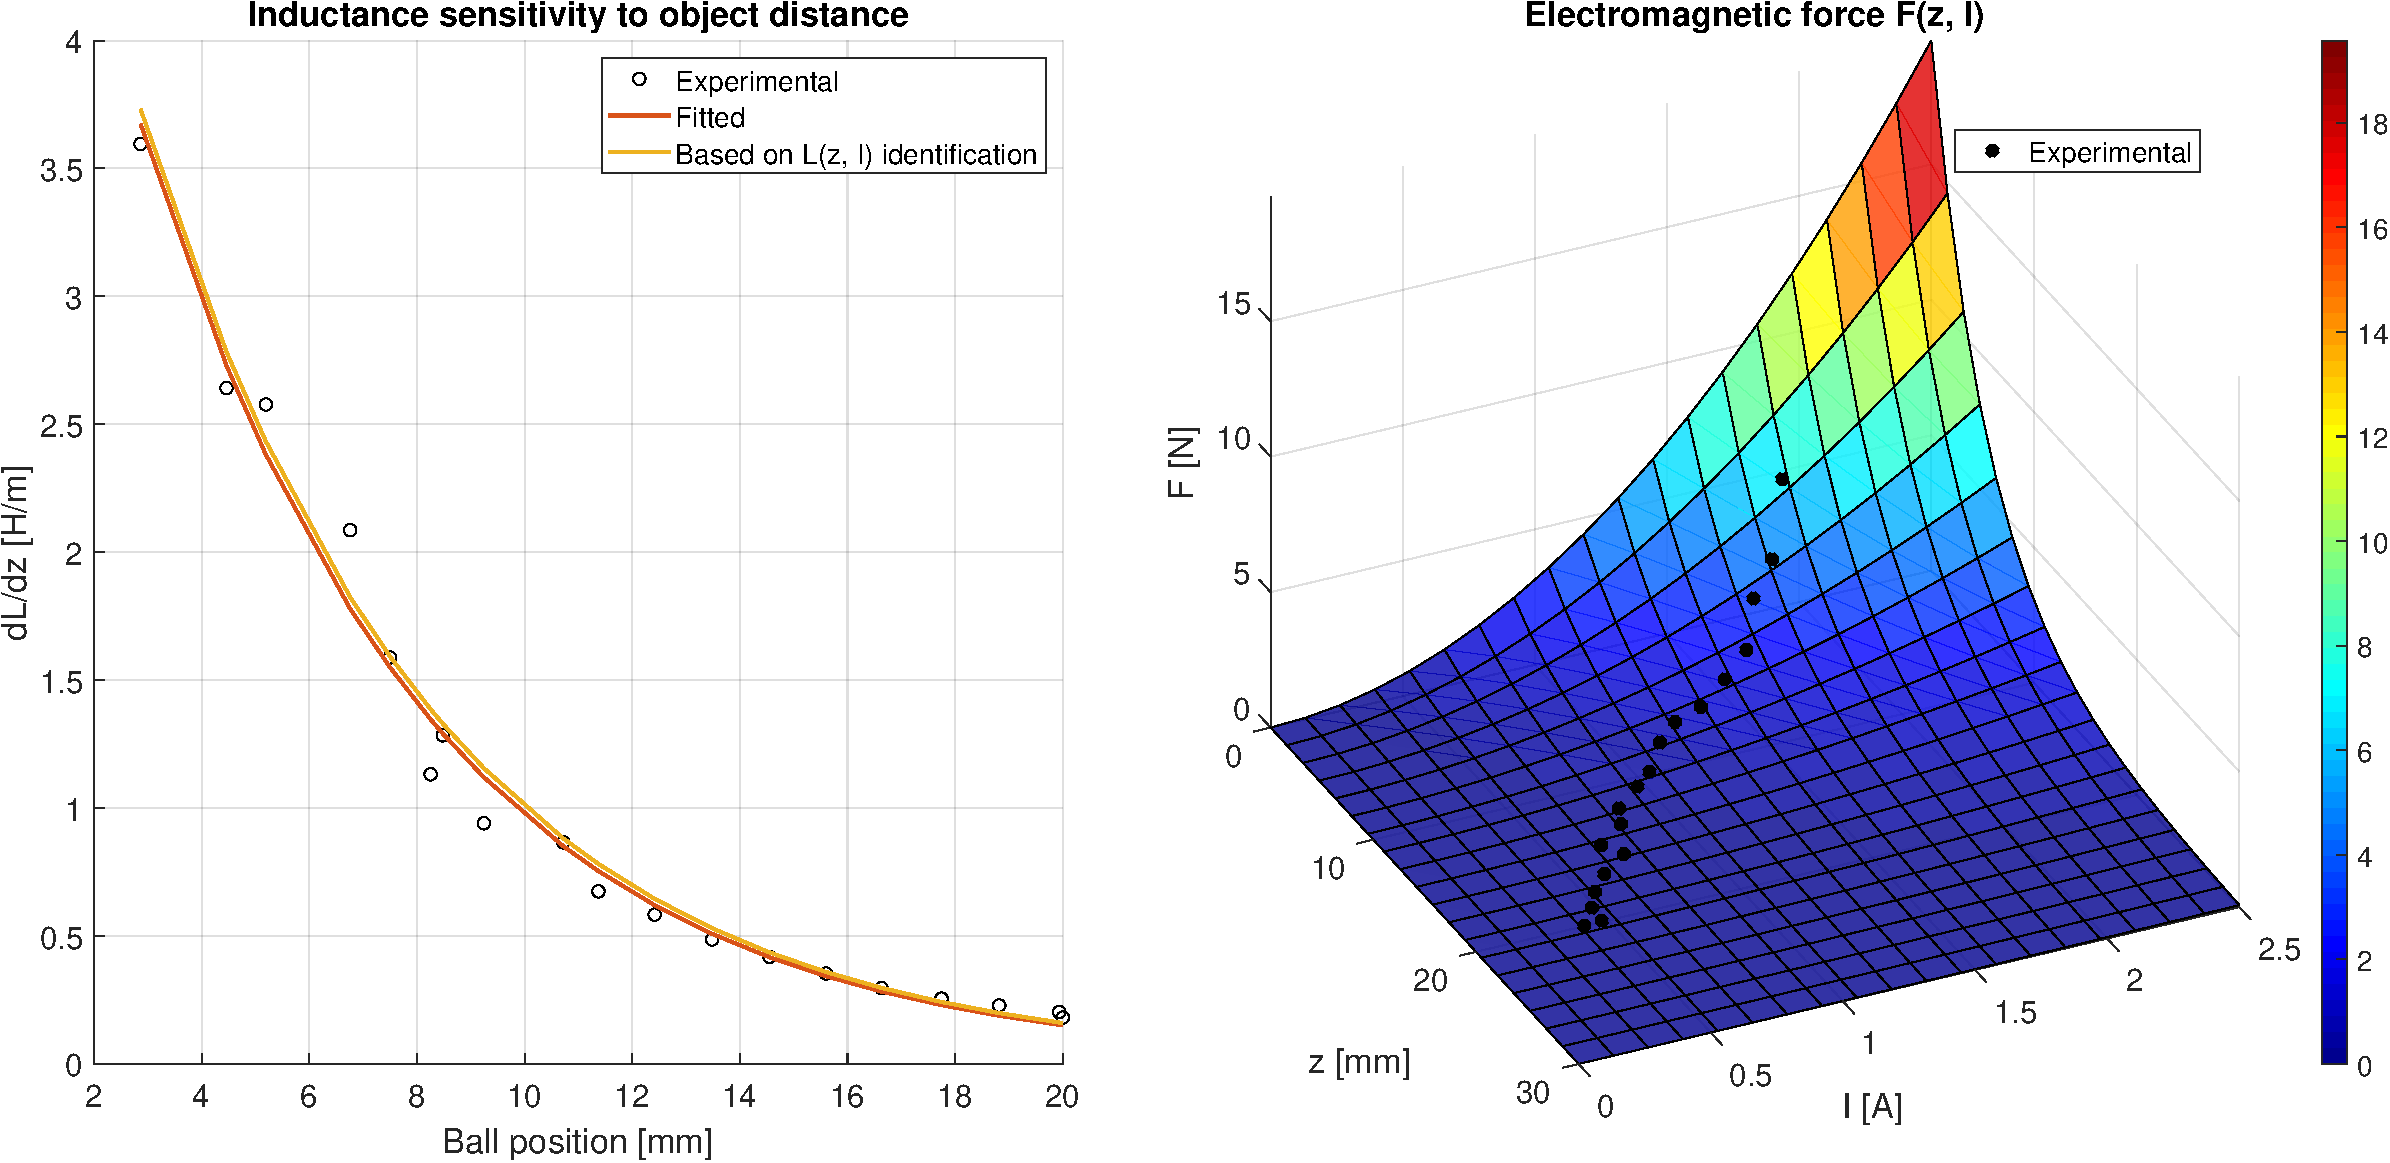
\includegraphics[width=0.8\textwidth]{img/MATLAB/identification/force.pdf}
                    \caption{Electromagnetic force as a function of $z$ and $I$}
                \end{figure}

            \end{column}

            \begin{column}{0.35\textwidth}

                Notice that from the theoretical model, we have found the electromagnetic force acting on the ball to be:

                \begin{equation}
                    F_{em} = \frac{1}{2} \frac{\partial L}{\partial z} I^2
                \end{equation}

            \end{column}

        \end{columns}

    }

\end{frame}
% \section{Model Analysis}

\begin{frame}{Linearization and Transfer function $G(s)$}

    Considering linearization around the position of $10 [mm]$, the following state-space representation of the system is obtained:

    \begin{equation}
        A =
        \begin{bmatrix}
            0    & 1 & 0      \\
            1555 & 0 & -20.63 \\
            0    & 0 & -35.55
        \end{bmatrix}
        \quad
        B =
        \begin{bmatrix}
            0 \\
            0 \\
            99.41
        \end{bmatrix}
    \end{equation}

    \begin{equation}
        C =
        \begin{bmatrix}
            1 & 0 & 0
        \end{bmatrix}
        \quad
        D =
        \begin{bmatrix}
            0
        \end{bmatrix}
    \end{equation}

    Based on this, the transfer function $G(s)$ of the system is given by:

    \begin{equation}
        G(s) = C \left( sI - A \right)^{-1} B + D = \frac{-2051}{s^3 + 35.56 s^2 - 1555 s - 5.53\cdot10^4}
    \end{equation}

\end{frame}



\begin{frame}{Stability analysis}

    \begin{columns}[c, onlytextwidth]

        \begin{column}{0.60\textwidth}

            \begin{figure}[H]
                \centering
                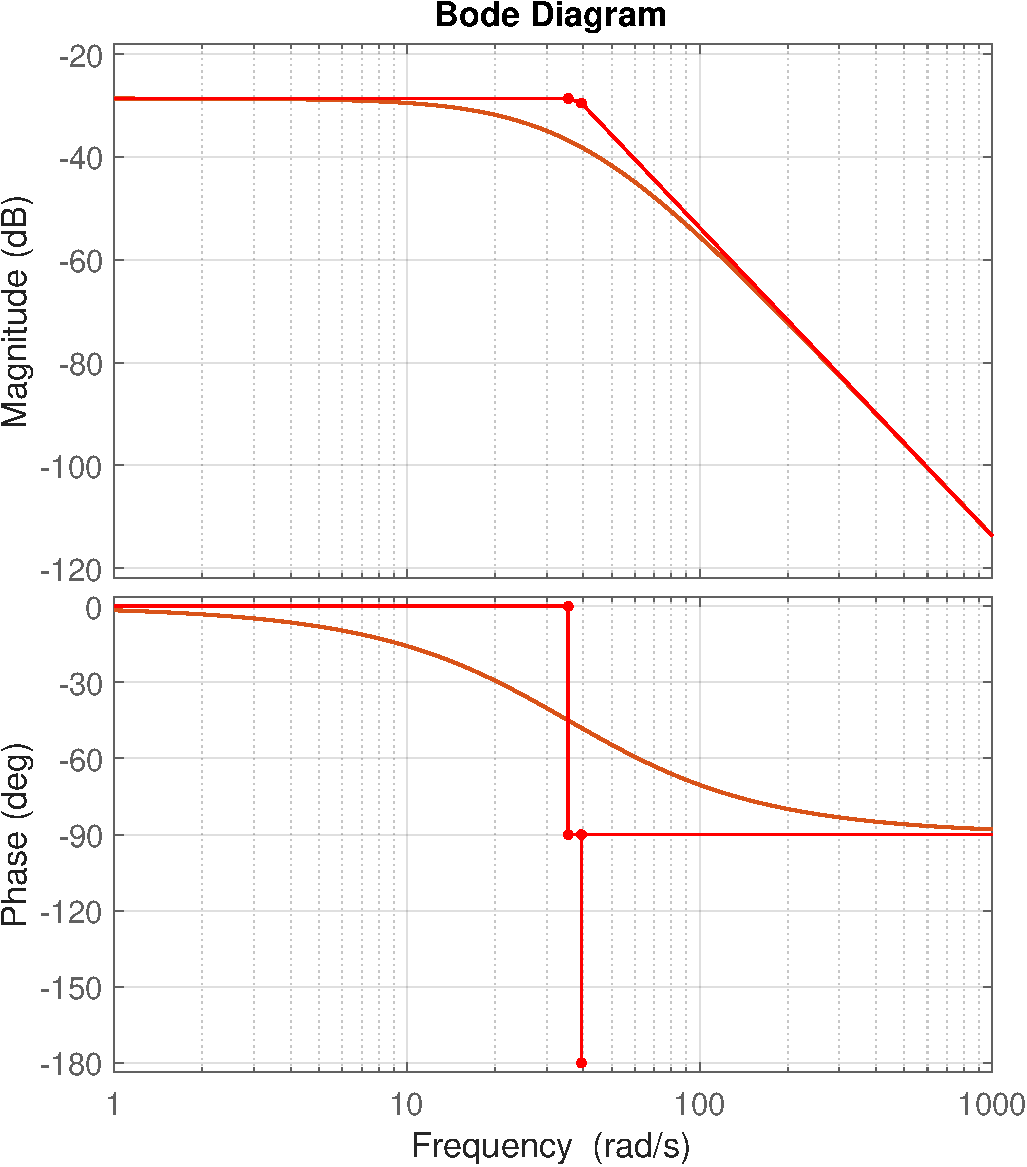
\includegraphics[width=0.8\textwidth]{./img/MATLAB/analysis/bode_plot_resized.pdf}
                \caption{Bode plot for the transfer function $G(s)$.}
            \end{figure}

        \end{column}

        \begin{column}{0.40\textwidth}

            The Bode plot shows that the system is unstable, as the gain margin is negative.

            \vspace{9pt}

            Instability is also confirmed by the poles of the system:

            \begin{equation}
                eig(A) =
                \begin{cases}
                    39.44  \\
                    -39.44 \\
                    -35.56
                \end{cases}
            \end{equation}

        \end{column}

    \end{columns}

\end{frame}



\begin{frame}{Stability analysis}

    \begin{figure}[H]
        \centering
        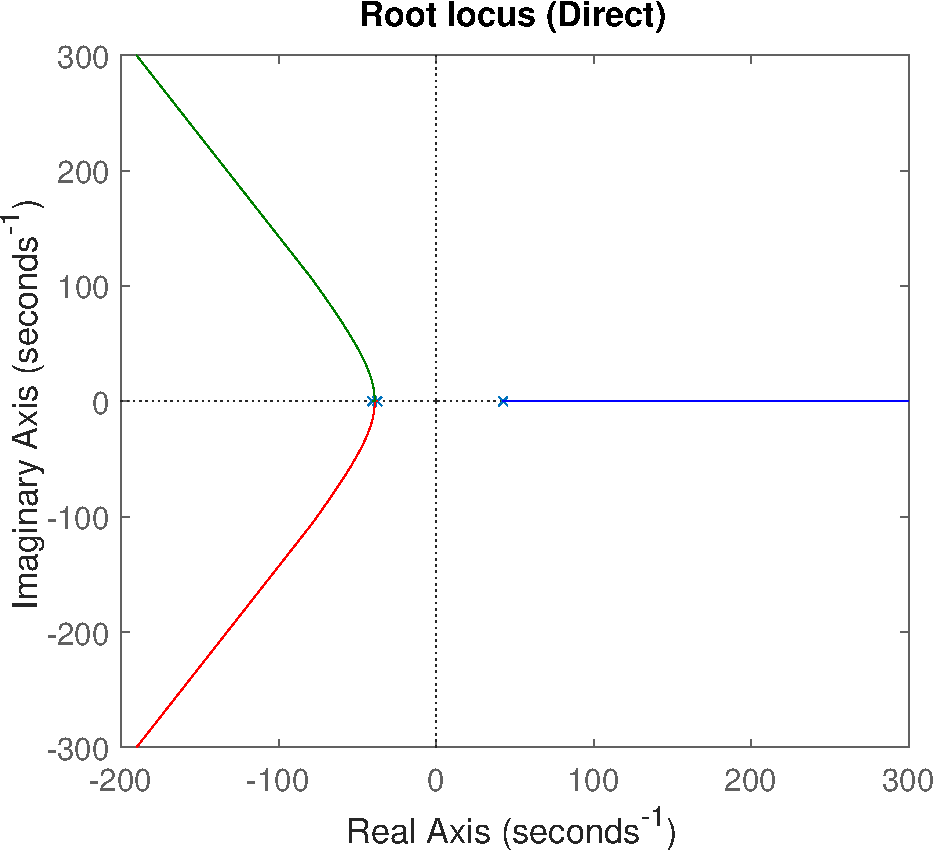
\includegraphics[width=0.47\textwidth]{./img/MATLAB/analysis/root_locus_direct.pdf}
        \hfill
        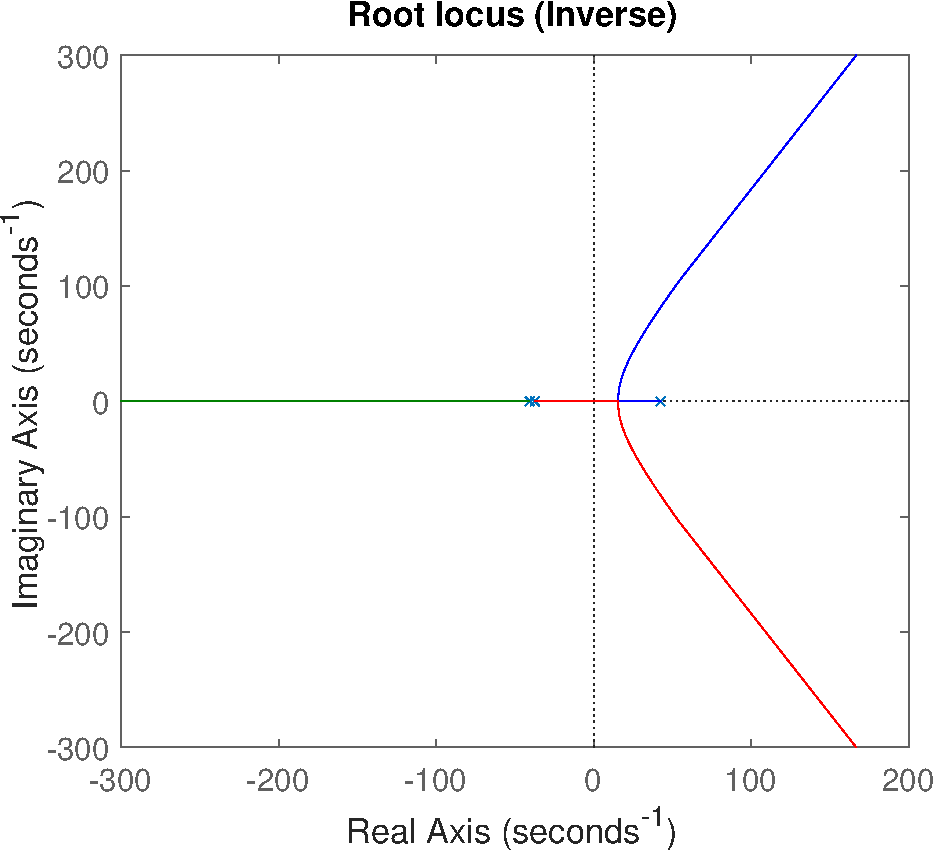
\includegraphics[width=0.47\textwidth]{./img/MATLAB/analysis/root_locus_inverse.pdf}
        \caption{Root Locus plot with positive and negative proportional feedback control.}
        \label{fig:root_locus_plot}
    \end{figure}


\end{frame}



\begin{frame}{Controllability and reachability}

    Luckily, the system is controllable and reachable, as the rank of both the controllability and reachability matrices is equal to the number of states.

    \vspace{9pt}

    We can now move on to the design of estimators and controllers for the system.

\end{frame}
% \section{Estimators and Filters Design}
\label{sec:filters_estimators_design}

\begin{frame}{Overview}

    Many control strategies require the knowledge of all the system states.
    For this reason, some state estimators have been designed together with some filters to reduce the noise in the measurements.

    \begin{itemize}
        \item \textbf{Low-pass filter};
        \item \textbf{Luenberger observer}.
        \item \textbf{Kalman filter}.
        \item \textbf{Extended Kalman filter}.
    \end{itemize}

\end{frame}

\begin{frame}{Low-pass filter}

    A first order low-pass filter has been implemented:

    \begin{equation}
        G(s) = \frac{1}{\tau s + 1}
    \end{equation}

    where the time constant of the filter is:

    \begin{equation}
        \tau = \frac{1}{\omega_c}=\frac{1}{200} = 5 ms
    \end{equation}

    where $\omega_c = 10 \omega_n \approx 200 rad/s$ is  the cut-off frequency, and $\omega_n = \frac{2\pi}{T_p} \approx 20 rad/s$ is the bandwidth of the system.
    Filter delay can also be computed as:

    \begin{equation}
        \phi = -artctan(\omega_c \tau) = -5.7^{\circ}
    \end{equation}

\end{frame}



\begin{frame}{Luenberger Observer}

    In order to estimate the state of the system\footnotemark[1], the Luenberger Observer has been implemented considering by chance the following eigenvalues:

    \begin{equation}
        eig(A-LC) =
        \begin{bmatrix}
            -500 \\
            -400 \\
            -400
        \end{bmatrix}
        \label{eq:luenberger_observer_poles}
    \end{equation}

    Leading to the following observer gain:

    \begin{equation}
        L =
        \begin{bmatrix}
            900.00    & 0      \\
            201555.32 & -20.63 \\
            0         & 364.44
        \end{bmatrix}
        \label{eq:L_luemberg}
    \end{equation}

    \footnotetext[1]{For all the estimators proposed, we consider to have both $z$ and $I$ as measurements from the system and estimate $v$.}

\end{frame}



\begin{frame}{Kalman filter}

    Another estimation of the state of the system can be made with the Kalman filter, where process and noise covariance matrices are given by:

    \begin{equation}
        Q = \begin{bmatrix}
            0 & 0  & 0  \\
            0 & 10 & 0  \\
            0 & 0  & 10
        \end{bmatrix}
        \quad
        R = \begin{bmatrix}
            7.21 \cdot 10^{-10} & 0                  \\
            0                   & 4.21 \cdot 10^{-5}
        \end{bmatrix}
    \end{equation}

    The Kalman gain $K$ is then obtained:

    \begin{equation}
        K = \begin{bmatrix}
            487    & -0  \\
            119069 & -15 \\
            -911   & 453
        \end{bmatrix}
        \label{eq:kalman_gain_matrix}
    \end{equation}

    the poles of the observer are given by:

    \begin{equation}
        eig(A - K C) =
        \begin{bmatrix}
            -243.94 + 240.82i \\
            -243.94 - 240.82i \\
            -488.87 + 0i
        \end{bmatrix}
        \label{eq:K_kalman}
    \end{equation}

\end{frame}



\begin{frame}{Extended Kalman filter}

    The extended Kalman filter does a recursive state estimation for our nonlinear systems.

    \vspace{9pt}

    The design parameters are the same as the Kalman filter with the key difference that the gain matrix $K_k$ is computed online at each time step $t_k$ based on the current state estimate $\hat{x}_k$.

\end{frame}
% \section{Controllers design}
\label{sec:controllers_design}

\begin{frame}{Overview}
    The control of the system is achieved by designing different controllers:
    \begin{itemize}
        \item \textbf{PIDs controller};
        \item \textbf{LQs controller};
        \item \textbf{MPC controller}.
    \end{itemize}
\end{frame}



\begin{frame}{PID with Anti-Windup}
    \normalsize
    \begin{itemize}
        \item \textbf{Problem}: \textbf{Integrator windup} occurs when the actuator saturates, causing uncontrolled growth of the integral term. This degrades the rise time and can lead to a \textbf{higher overshoot}.
        \item \textbf{Solution}: \textbf{Conditional Integration}. The controller output is compared with the actuator limits. If saturation is detected and error accumulates, the integrator is \textbf{turned off}.
    \end{itemize}

    The gain parameters reported below have been estimated firstly considering the Bode diagram, and subsequently analyzing the Root Locus:
    \begin{equation}
        K_p = -150 \quad K_i = -450 \quad K_d = -6.82
    \end{equation}
\end{frame}



\begin{frame}{PID with Gain Scheduling}

    \begin{itemize}
        \item \textbf{PID controller} tuned at a series of \textbf{steady-state operating points}.
        \item The sphere's movement space is divided into \textbf{multiple points}, and the system is \textbf{linearized} locally at each operating point.
        \item Controller gains are \textbf{optimized} for each operating condition.
        \item Gain curves \textbf{gradually vary} between points.
    \end{itemize}

    \begin{table}[H]
        \centering
        \begin{tabular}{|c|c|c|c|}
            \hline
            $z [mm]$ & $K_p$  & $K_i$   & $K_d$   \\
            \hline
            $5$      & $-102$ & $-306$  & $-4.64$ \\
            $8$      & $-136$ & $-408$  & $-6.18$ \\
            $12$     & $-183$ & $-550$  & $-8.34$ \\
            $16$     & $-250$ & $-750$  & $-11.4$ \\
            $20$     & $-342$ & $-1030$ & $-15.5$ \\
            \hline
        \end{tabular}
        \caption{Look up table for the PID gain scheduling}
        \label{tab:pid_gain_scheduling_gains}
    \end{table}
\end{frame}



\begin{frame}{LQR with tracking capabilities}

    \textbf{The LQR with tracking capabilities}, extends the classical LQR framework to manage systems where the goal is not only to stabilize the system but also to ensure it follows a desired trajectory.

    For the matrix $\mathbf{Q}$, particular attention is given to the values affecting the position of the sphere, with moderate emphasis on the current state.
    The matrix $\mathbf{R}$ is estimated based on literature parameters.

    \begin{itemize}
        \item \textbf{Design parameters:}
              \begin{equation}
                  \mathbf{Q} =
                  \begin{bmatrix}
                      25\cdot10^3 & 0 & 0              \\
                      0           & 0 & 0              \\
                      0           & 0 & 16\cdot10^{-2}
                  \end{bmatrix}
                  \quad
                  \mathbf{R} = 0.5
              \end{equation}

        \item \textbf{Computed feedback gain:}
              \begin{equation}
                  \mathbf{K} =
                  \begin{bmatrix}
                      -371.72 & -7.53 & 1.53
                  \end{bmatrix}
              \end{equation}
    \end{itemize}
\end{frame}



\begin{frame}{LQI}

    \textbf{The LQI (Linear Quadratic Integrator)} is an extension of LQR that incorporates integral states to improve reference tracking and disturbance rejection.
    By adding integration of tracking error, LQI reduces persistent errors between the system and reference, improving control accuracy.

    \begin{itemize}
        \item \textbf{Design parameters:}
              \begin{equation}
                  \mathbf{Q} = \begin{bmatrix}
                      25\cdot10^3 & 0 & 0              & 0    \\
                      0           & 0 & 0              & 0    \\
                      0           & 0 & 16\cdot10^{-2} & 0    \\
                      0           & 0 & 0              & 10^6
                  \end{bmatrix} \quad \mathbf{R} = 0.5
              \end{equation}
        \item \textbf{Computed feedback gain:}
              \begin{equation}
                  \mathbf{K} = \begin{bmatrix}
                      -513.31 & -9.19 & 1.71 & 4472.13
                  \end{bmatrix}
              \end{equation}
    \end{itemize}
\end{frame}



\begin{frame}{MPC}

    \textbf{Model Predictive Control (MPC)} is an advanced control strategy that optimizes system performance by continuously reinitializing the control procedure.

    \begin{itemize}
        \item Based on a linear system model.
        \item Constraints are applied.
        \item Computationally less expensive compared to nonlinear MPC.
    \end{itemize}

    \begin{equation}
        \begin{aligned}
            \textbf{Prediction Horizon} & = 0.1 \, \text{s}  \\
            \textbf{Control Horizon}    & = 0.01 \, \text{s}
        \end{aligned}
    \end{equation}

    Constraints on position and control are applied, as shown in the table below:

    \begin{table}[H]
        \centering
        \begin{tabular}{|c|c|c|}
            \hline
            \textbf{Variable} & \textbf{Max} & \textbf{Min} \\
            \hline
            Position          & 20 mm        & 0 mm         \\
            \hline
            Control           & 1            & 0            \\
            \hline
        \end{tabular}
        \caption{Constraints for the MPC controller}
    \end{table}
\end{frame}

% \section{Results}

\begin{frame}{Controller comparison}

    Different reference signals have been used to evaluate the controllers' performance, including:

    \begin{itemize}
        \item \textbf{Multistep (stars and up \& down)}: a sequence of equally spaced step inputs ($1[mm]$ or $2[mm]$ in amplitude) to assess the controller's response to abrupt set-point changes and its steady-state performance across various set-points.
        \item \textbf{Sinusoidal (discrete)}: a sinusoidal shape (period $2[s]$, amplitude $2[mm]$), but represented as a sequence of discrete steps, to evaluate the controllers' performance in tracking a periodic signal.
    \end{itemize}

    \vspace{9pt}

    All the results here presented are obtained using a Kalman filter to estimate and/or filter the system's state.

\end{frame}



\begin{frame}{Controller comparison}

    \vspace{9pt}

    \begin{figure}[H]
        \centering
        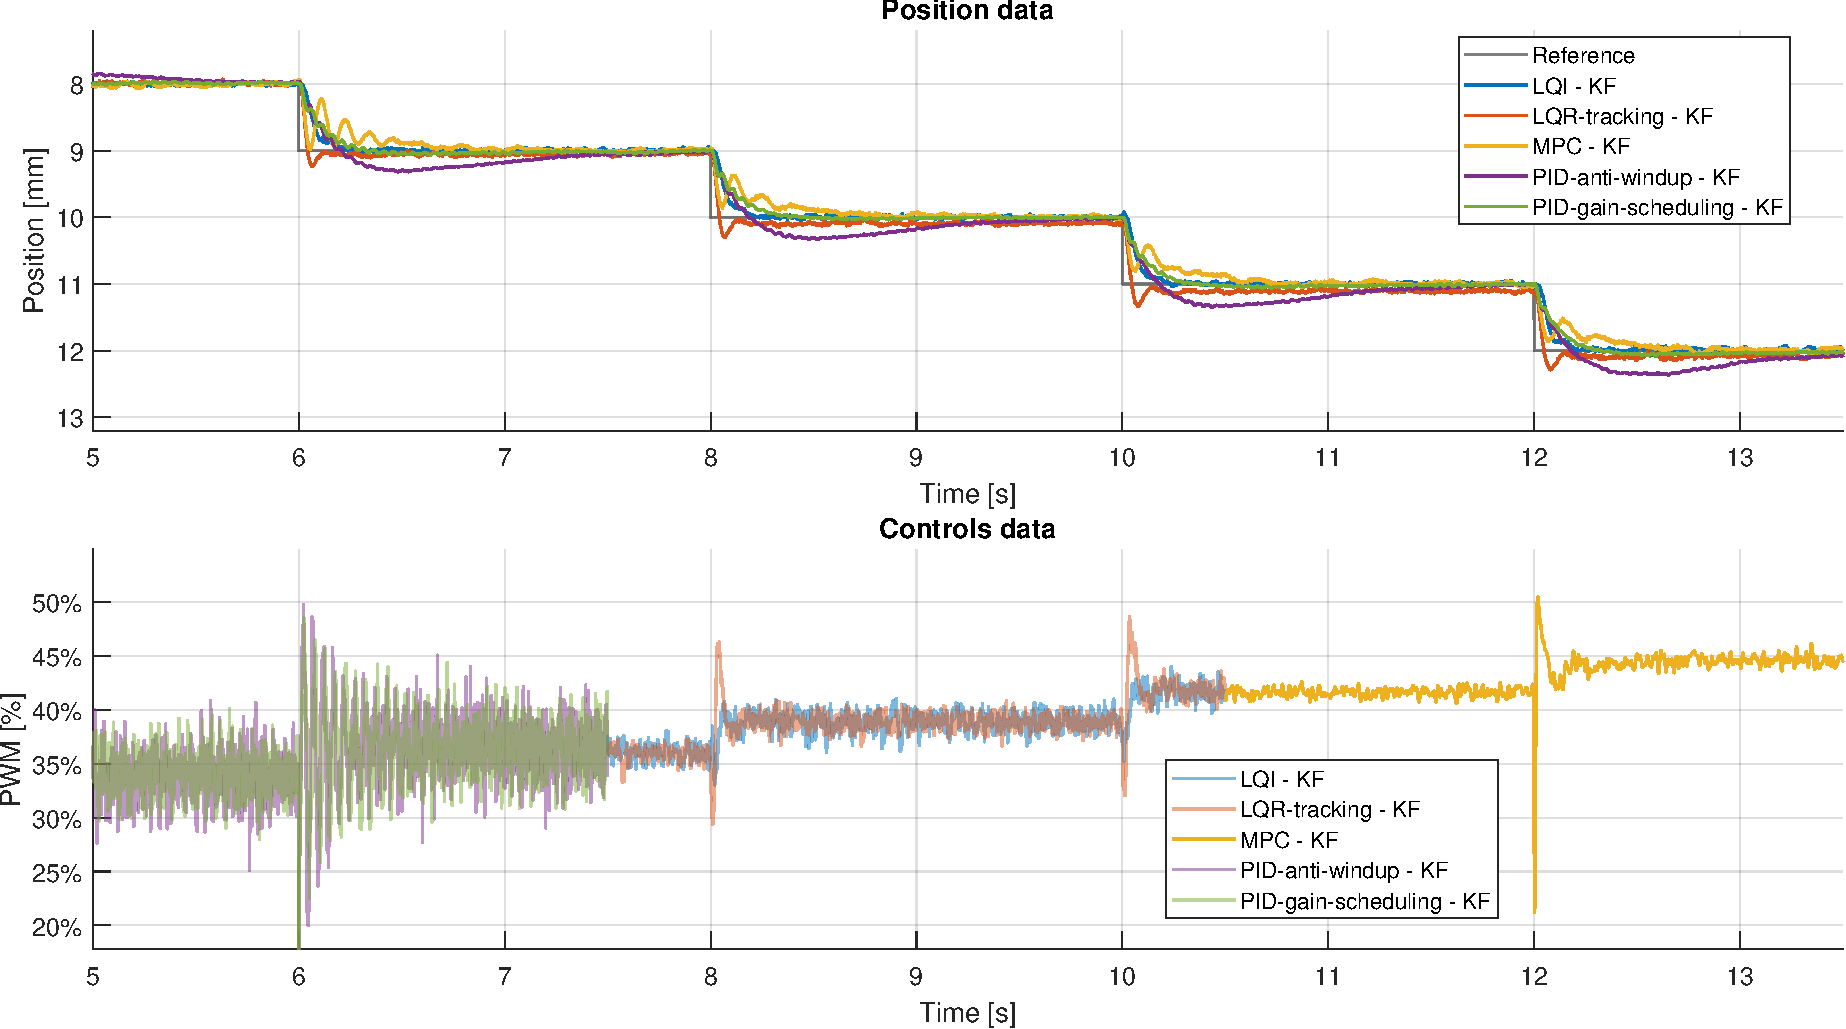
\includegraphics[width=1\linewidth]{./img/MATLAB/results/multisteps_stairs_star_KF.pdf}
        \caption{Comparison of controllers with multistep stairs reference using KF}
    \end{figure}

\end{frame}



\begin{frame}{Controller comparison}

    \vspace{9pt}

    \begin{figure}[H]
        \centering
        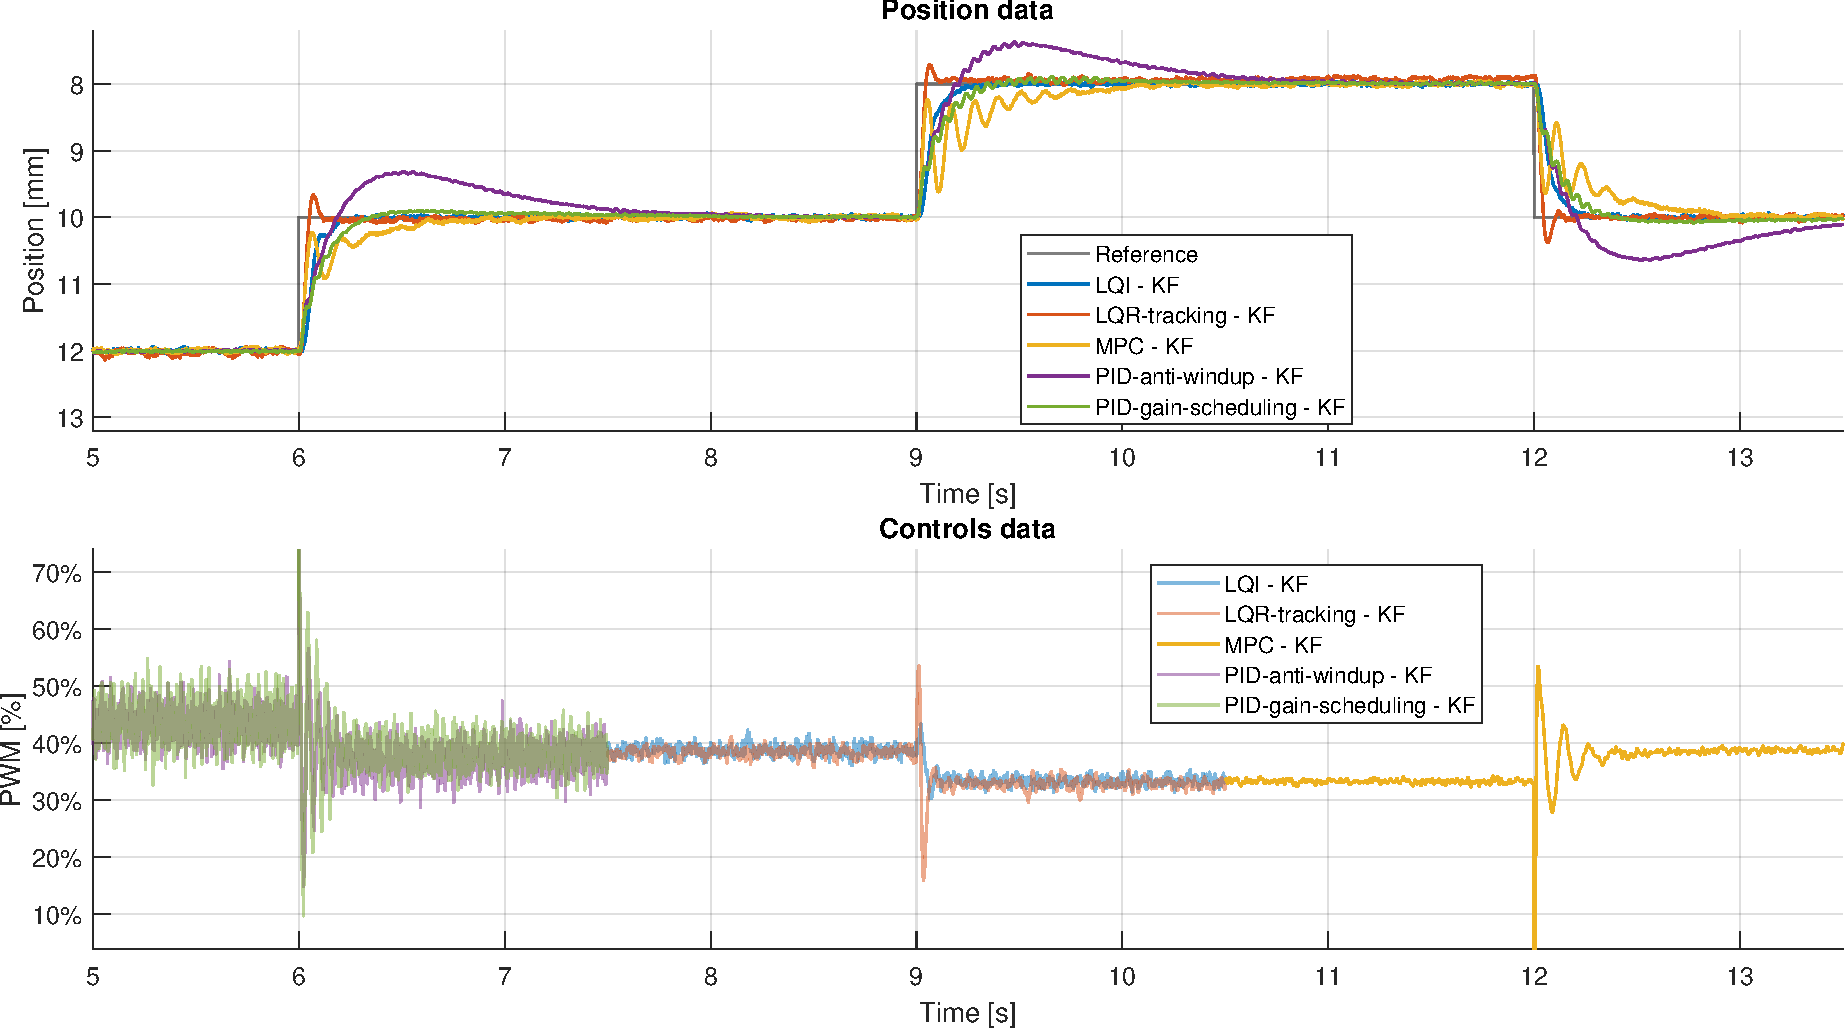
\includegraphics[width=1\linewidth]{./img/MATLAB/results/multisteps_updown_star_KF.pdf}
        \caption{Comparison of controllers with multistep up \& down reference using KF}
    \end{figure}

\end{frame}



\begin{frame}{Controller comparison}

    \vspace{9pt}

    \begin{figure}[H]
        \centering
        \onslide<1->{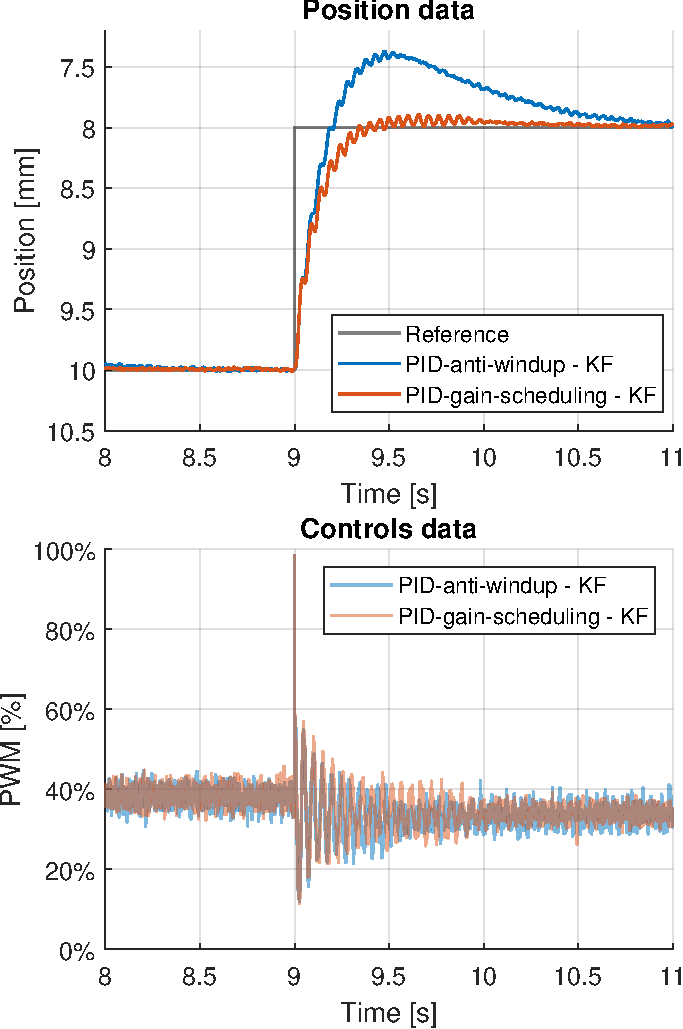
\includegraphics[width=0.32\linewidth]{./img/MATLAB/results/multisteps_up_PIDstar_KF.pdf}}
        \hfill
        \onslide<2->{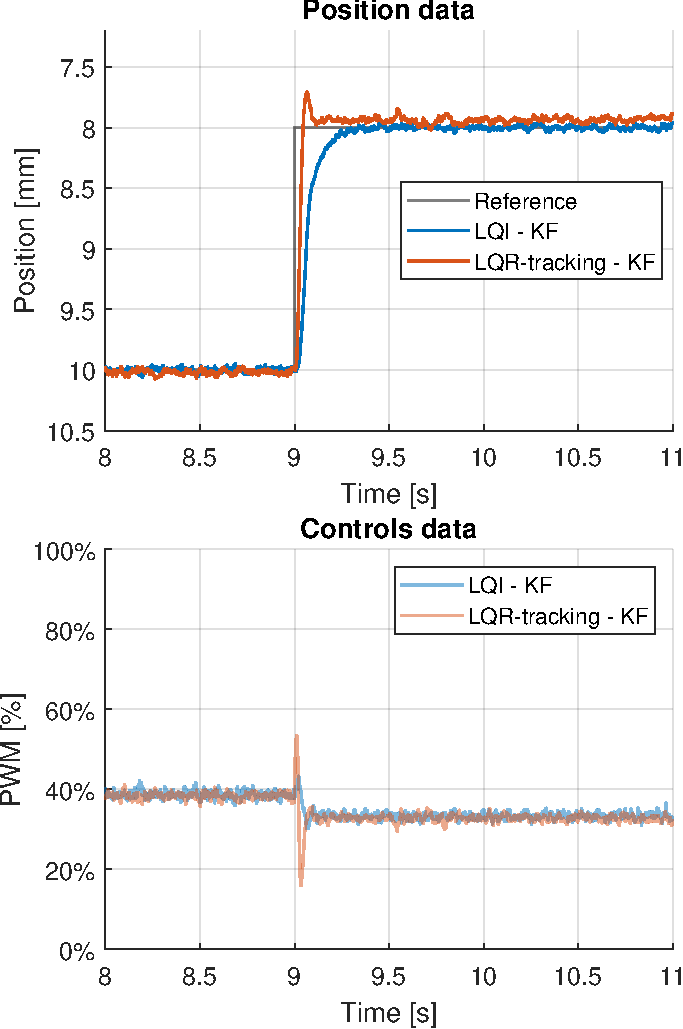
\includegraphics[width=0.32\linewidth]{./img/MATLAB/results/multisteps_up_LQstar_KF.pdf}}
        \hfill
        \onslide<3->{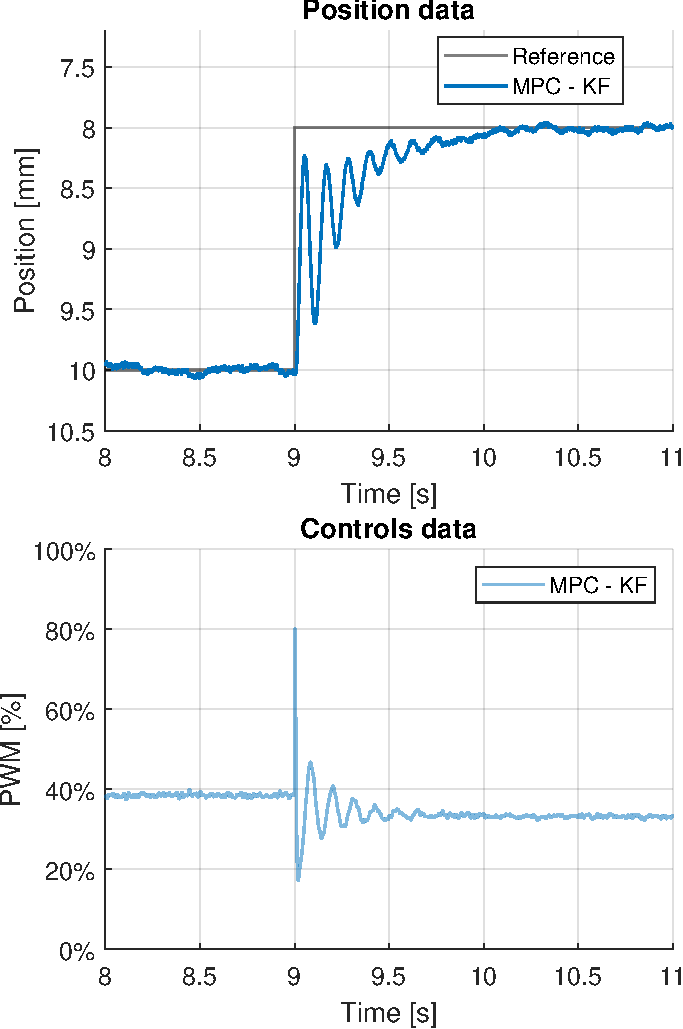
\includegraphics[width=0.32\linewidth]{./img/MATLAB/results/multisteps_up_MPCstar_KF.pdf}}
        \caption{PIDs, LQs, MPC with multistep up reference using KF}
    \end{figure}

\end{frame}



\begin{frame}{Controller comparison}

    \vspace{9pt}

    \begin{figure}[H]
        \centering
        \onslide<1->{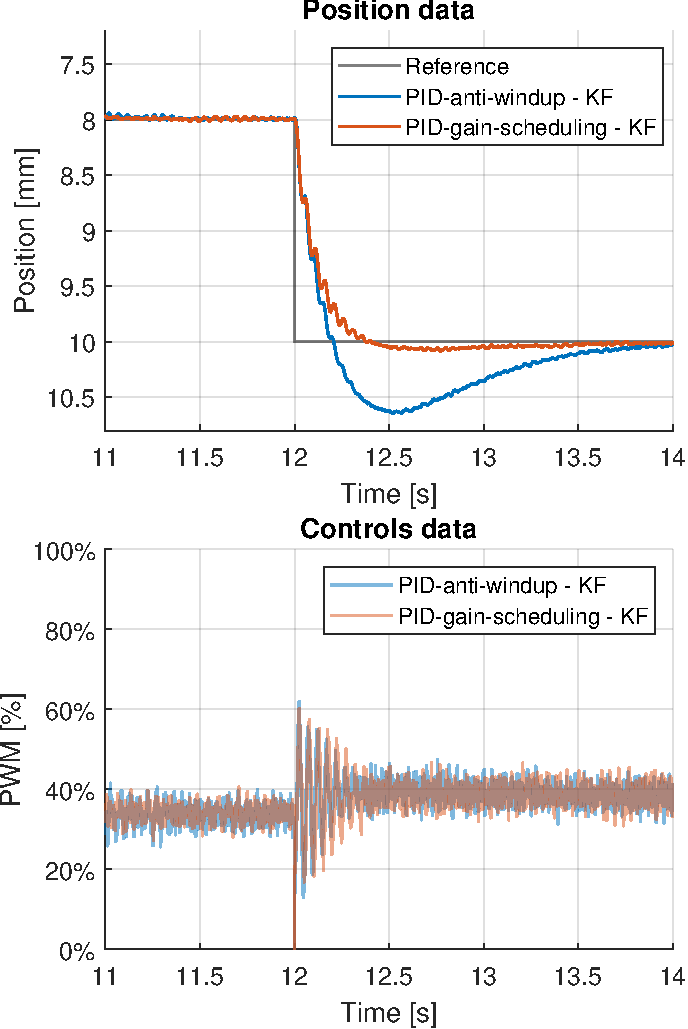
\includegraphics[width=0.32\linewidth]{./img/MATLAB/results/multisteps_down_PIDstar_KF.pdf}}
        \hfill
        \onslide<2->{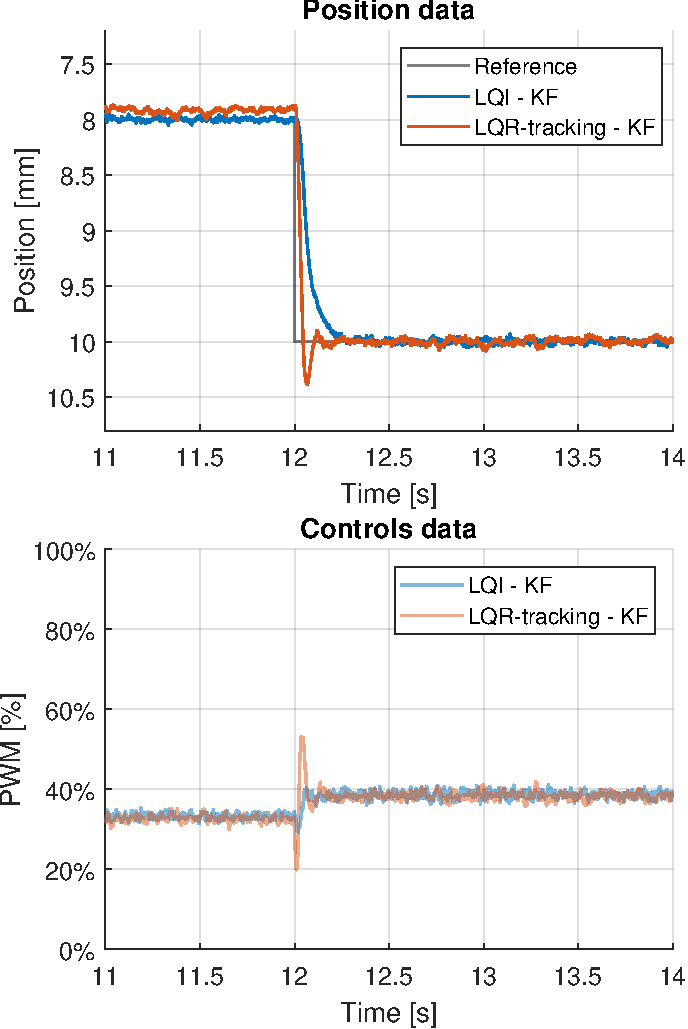
\includegraphics[width=0.32\linewidth]{./img/MATLAB/results/multisteps_down_LQstar_KF.pdf}}
        \hfill
        \onslide<3->{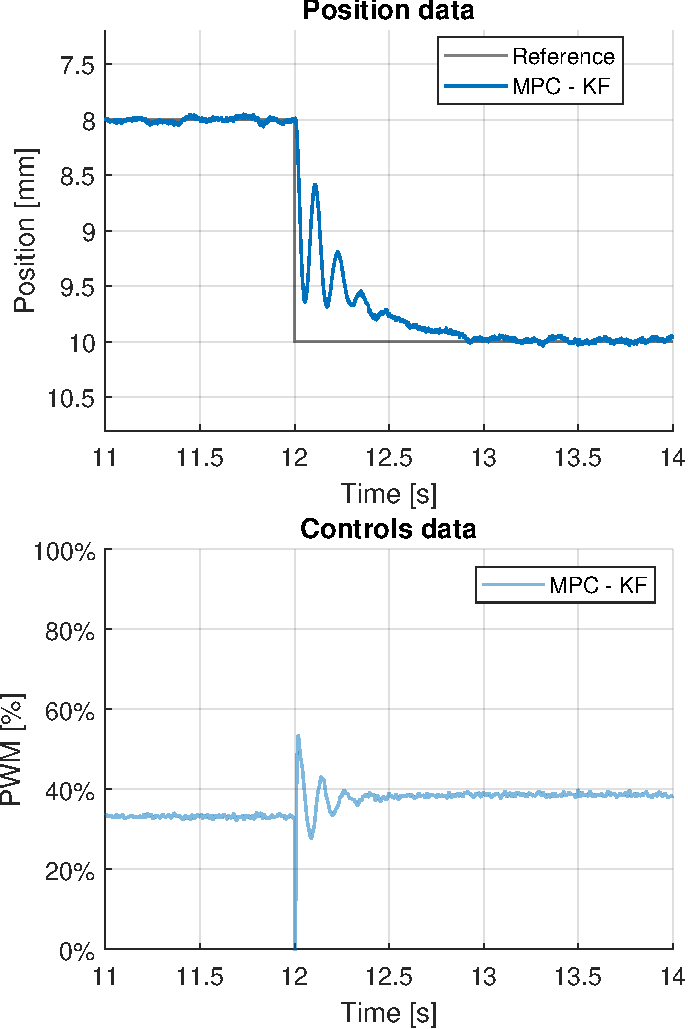
\includegraphics[width=0.32\linewidth]{./img/MATLAB/results/multisteps_down_MPCstar_KF.pdf}}
        \caption{PIDs, LQs, MPC with multistep up \& down (down) reference using KF}
    \end{figure}

\end{frame}



\begin{frame}{Controller comparison}

    \vspace{9pt}

    \begin{figure}[H]
        \centering
        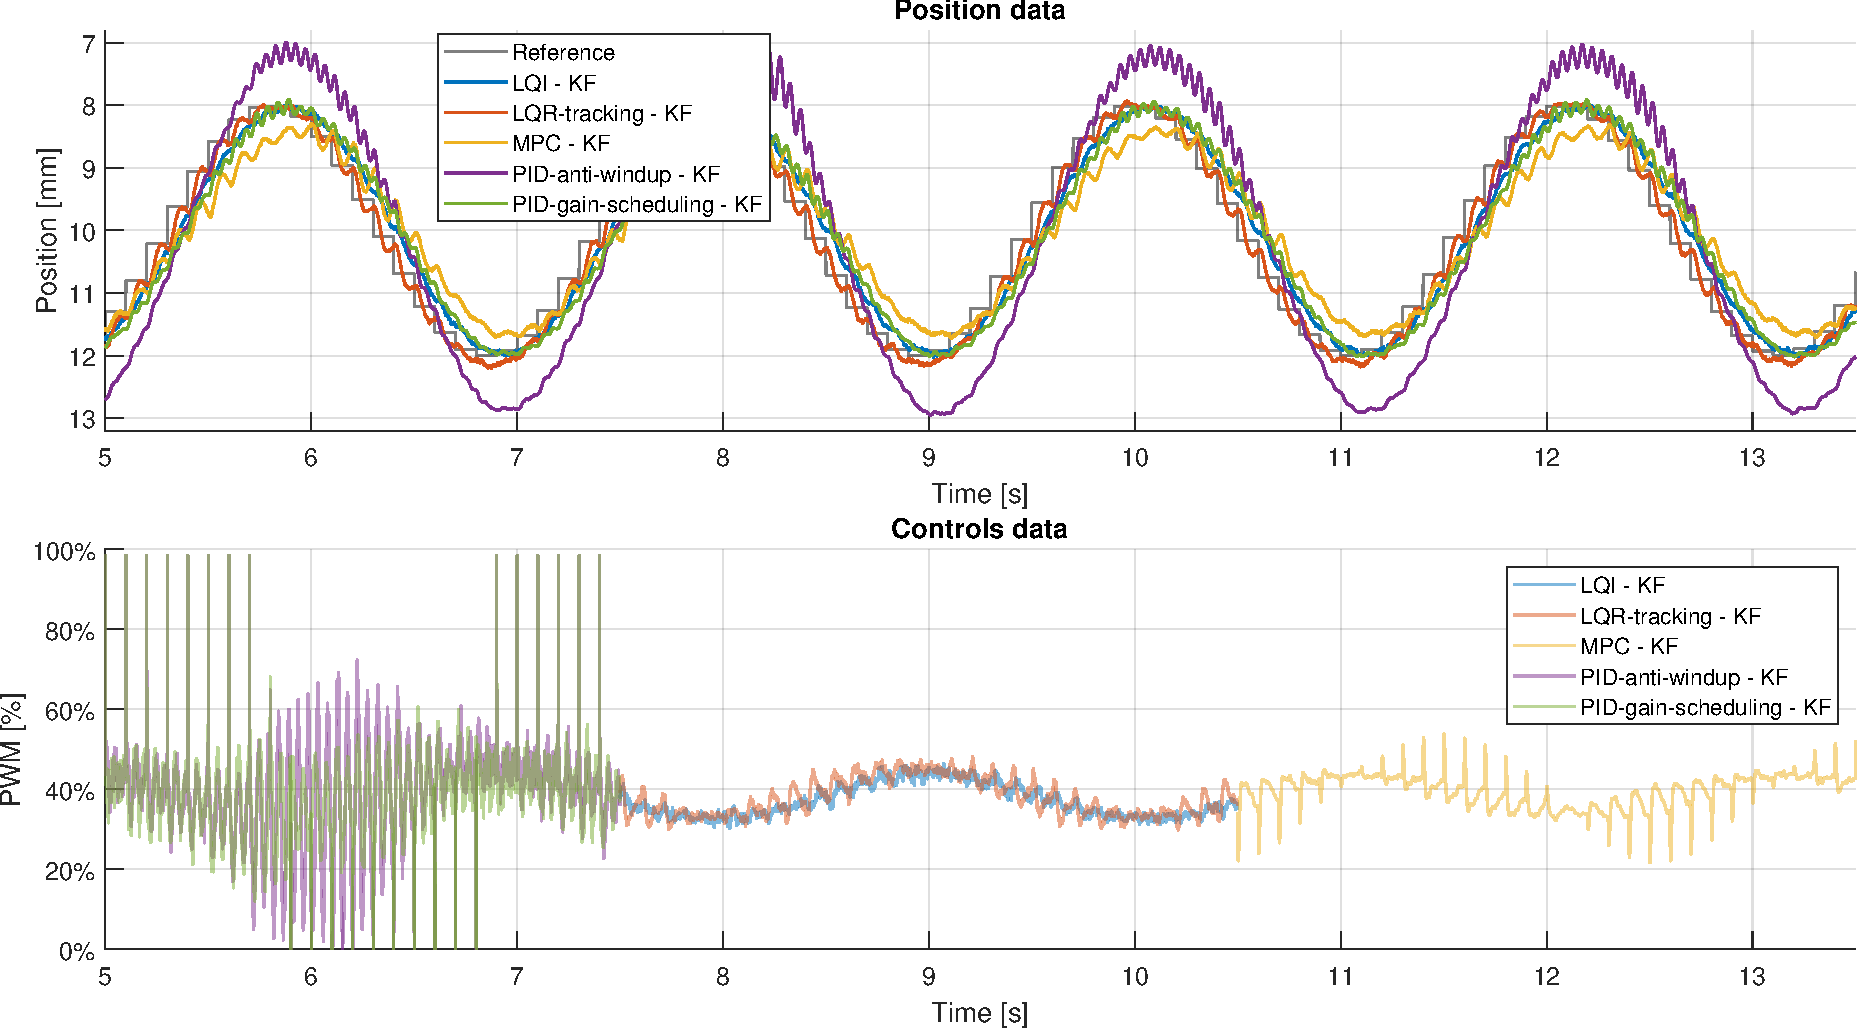
\includegraphics[width=1\linewidth]{./img/MATLAB/results/sinusoidal_fast_star_KF.pdf}
        \caption{Comparison of controllers with sinusoidal slow reference using KF}
    \end{figure}

\end{frame}



\begin{frame}{Controller comparison}

    \vspace{9pt}

    \begin{figure}[H]
        \centering
        \onslide<1->{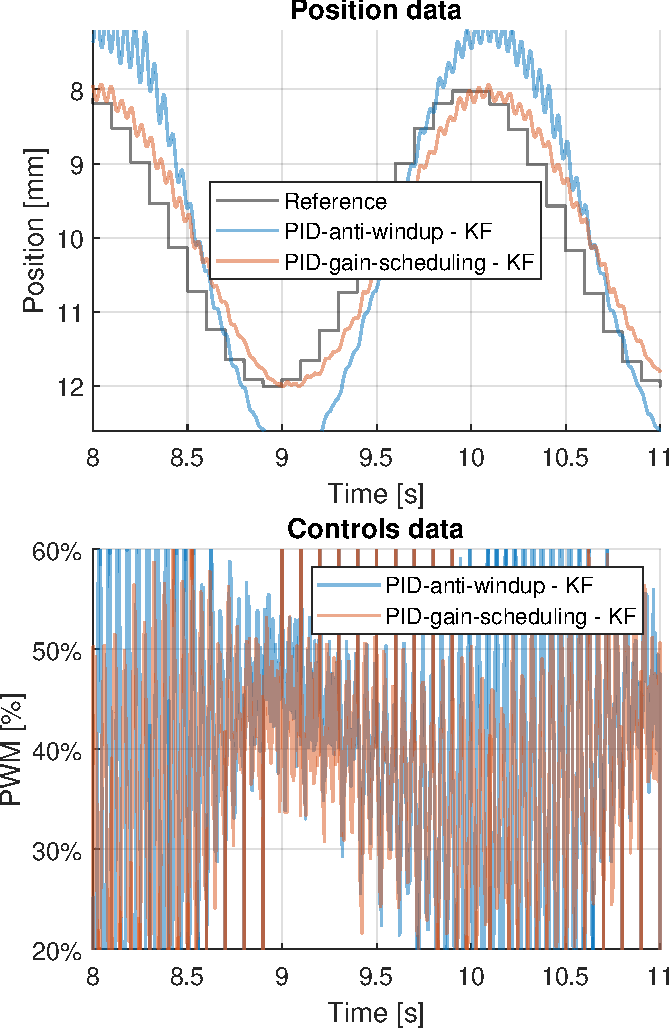
\includegraphics[width=0.32\linewidth]{./img/MATLAB/results/sinusoidal_fast_PIDstar_KF.pdf}}
        \hfill
        \onslide<2->{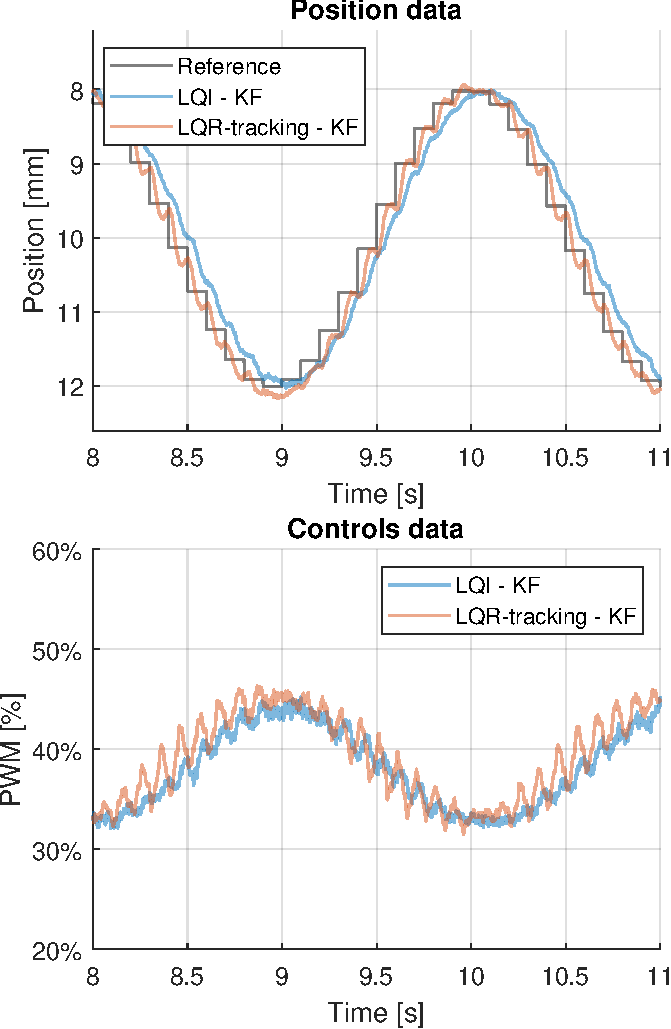
\includegraphics[width=0.32\linewidth]{./img/MATLAB/results/sinusoidal_fast_LQstar_KF.pdf}}
        \hfill
        \onslide<3->{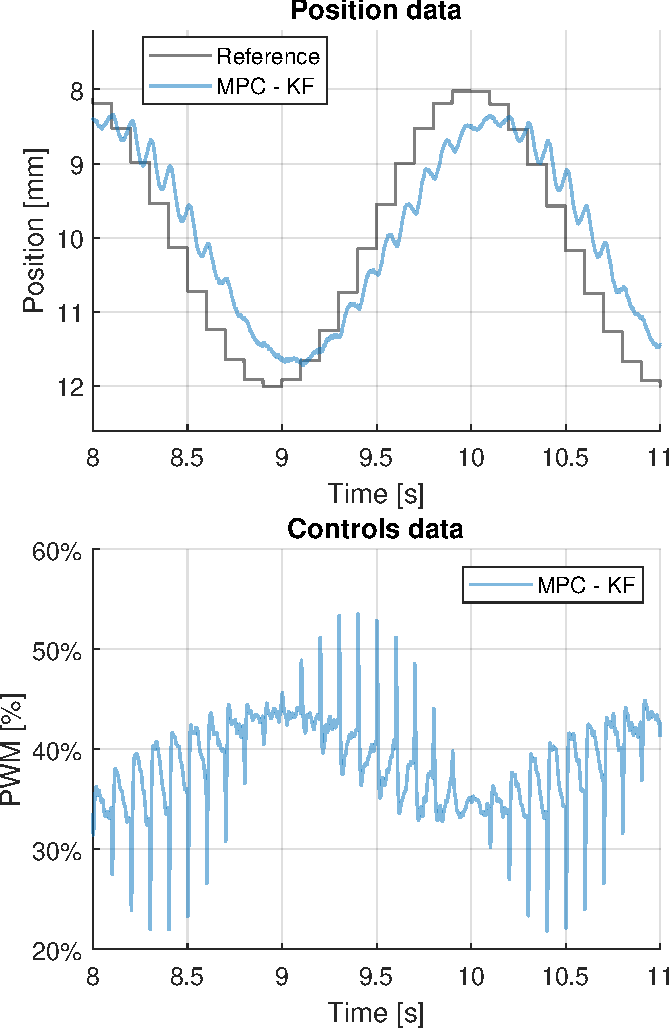
\includegraphics[width=0.32\linewidth]{./img/MATLAB/results/sinusoidal_fast_MPCstar_KF.pdf}}
        \caption{PIDs, LQs, MPC with sinusoidal fast reference using KF}
    \end{figure}

\end{frame}



\begin{frame}{Controller considerations}

    Overall, from the results obtained, we can draw the following considerations:

    \begin{table}[H]
        \centering
        \renewcommand{\arraystretch}{1}
        \begin{tabular}{|l|c|c|c|c|l|}
            \hline
            \textbf{Controller}          & \textbf{Reactivity} & \textbf{Precision}  & \textbf{Stability} & \textbf{Control} \\ \hline
            \textbf{PID Anti-windup}     & Slow                & Good (steady-state) & Moderate           & High noise       \\ \hline
            \textbf{PID Gain Scheduling} & Good                & Good                & Good               & High noise       \\ \hline
            \textbf{LQR Tracking}        & Very high           & High                & Good               & Very Good        \\ \hline
            \textbf{LQI}                 & Very high           & Excellent           & Excellent          & Excellent        \\ \hline
            \textbf{MPC}                 & High                & Good                & Good               & Good             \\ \hline
        \end{tabular}
        \caption{Controller Comparison}
    \end{table}


\end{frame}


\begin{frame}{Filter \& Estimator comparison}

    To compare filters and estimators, an LQR tracking was used as a controller and a continuous sinusoidal reference signal with a period of $2[s]$ and amplitude of $2[mm]$ was used as a reference signal.

    \vspace{9pt}

    Regarding the estimators, only position and current measurements were used as input, while velocity was estimated.

\end{frame}


\begin{frame}{Filter \& Estimator comparison}

    \vspace{9pt}

    \begin{figure}[H]
        \centering
        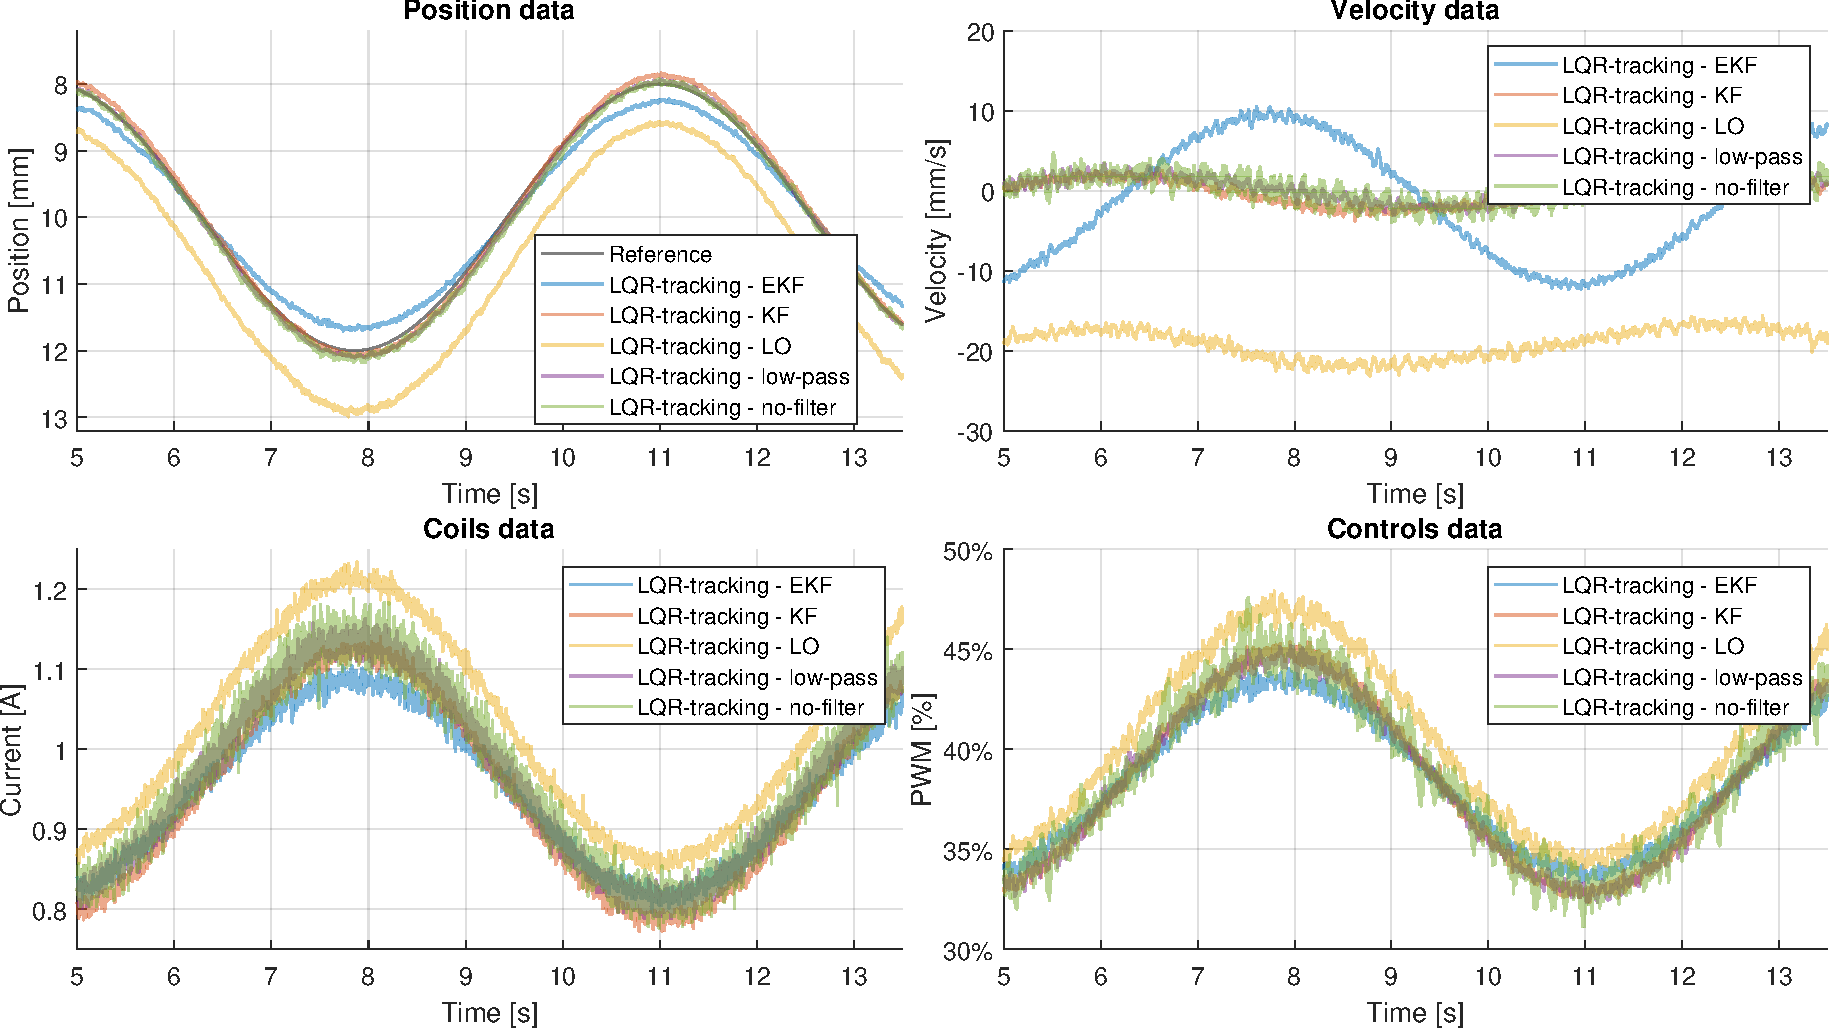
\includegraphics[width=1\linewidth]{./img/MATLAB/results/sinusoidal_slow_linear_star_star.pdf}
        \caption{Comparison of filter using an LQR tracking with sinusoidal slow reference}
    \end{figure}

\end{frame}



\begin{frame}{Filter \& Estimator comparison}

    \vspace{9pt}

    \begin{figure}[H]
        \centering
        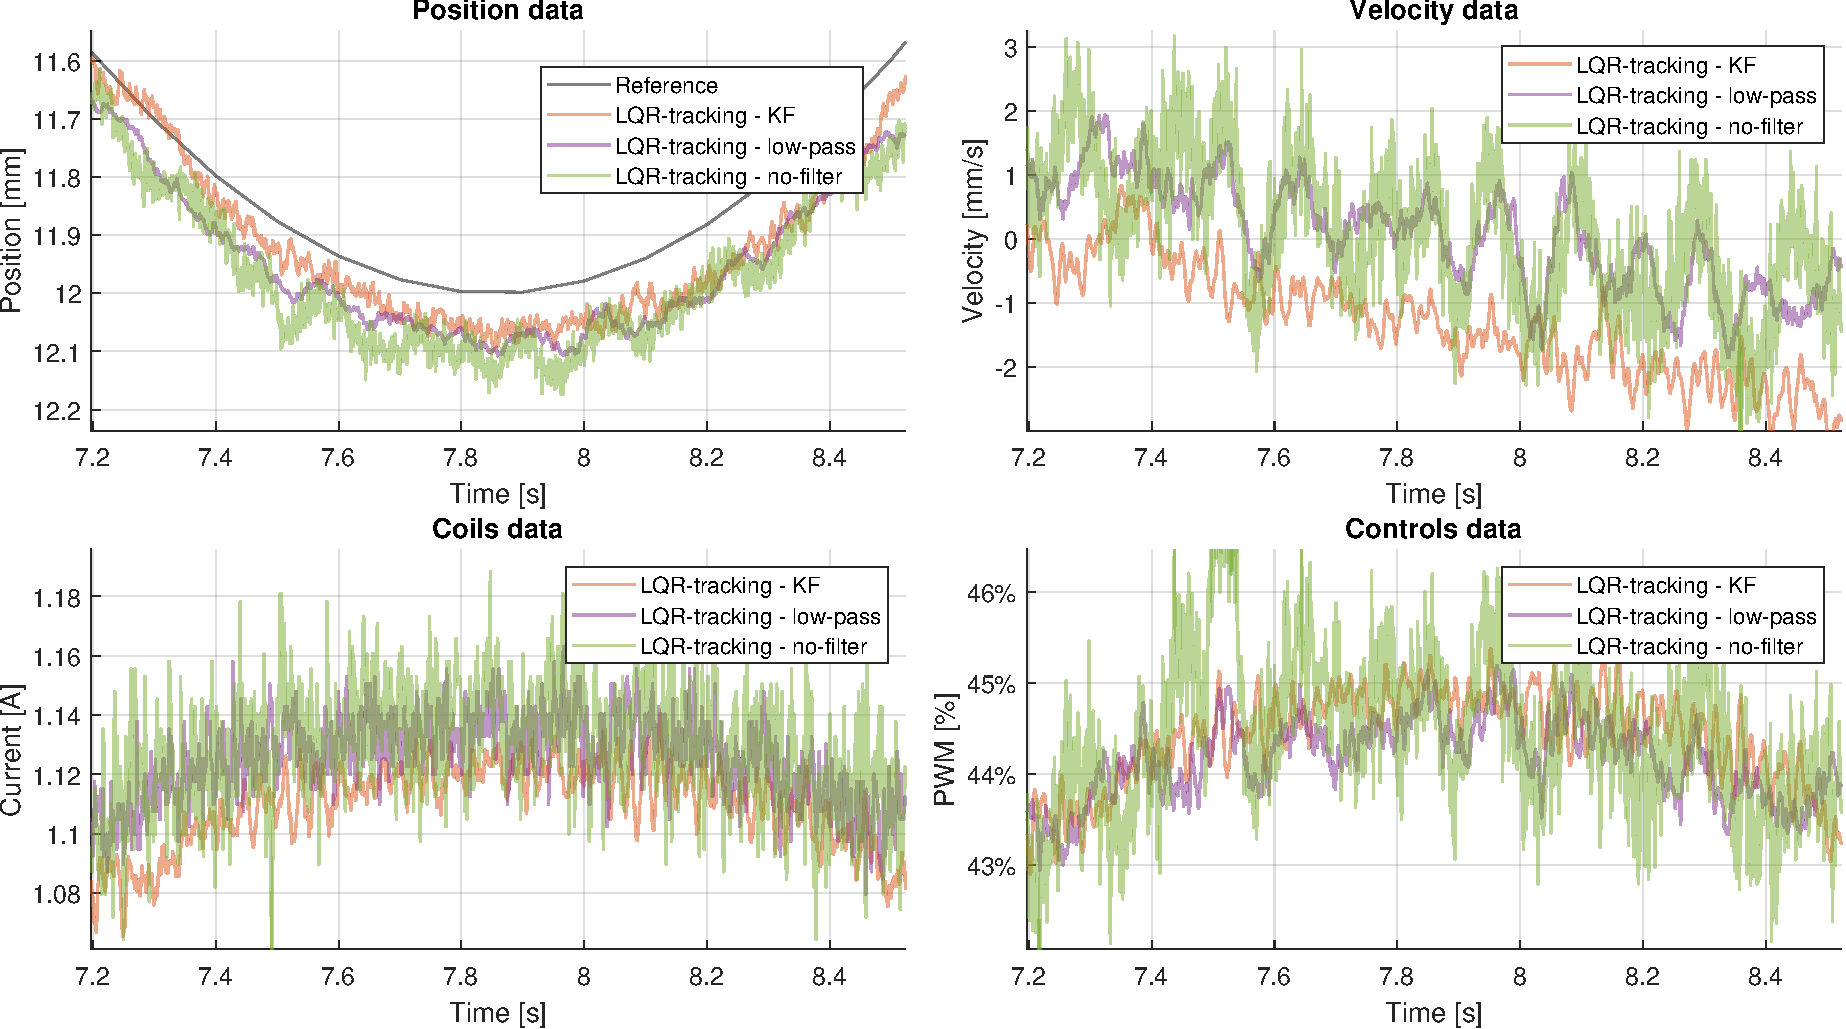
\includegraphics[width=1\linewidth]{./img/MATLAB/results/sinusoidal_slow_linear_zoomed_star_no_filter_low_pass_KF.pdf}
        \caption{Comparison of no filter, low pass, KF using an LQR tracking with sinusoidal slow reference}
    \end{figure}

\end{frame}



\begin{frame}{Filter \& Estimator considerations}

    Overall, from the results obtained, we can draw the following considerations:

    \begin{table}[H]
        \centering

        \begin{tabular}{|l|c|c|c|}
            \hline
            \textbf{Filter/Estimator}       & \textbf{Noise reduction} & \textbf{Estimation accuracy} & \textbf{Delay} \\ \hline
            \textbf{No filter}              & -                        & -                            & Absent         \\ \hline
            \textbf{Low-pass filter}        & Optimal                  & -                            & Minimal        \\ \hline
            \textbf{Luenberg Observer}      & Good                     & Extremely inaccurate         & Absent         \\ \hline
            \textbf{Kalman filter}          & Good                     & Good                         & Absent         \\ \hline
            \textbf{Extended Kalman filter} & Good                     & Inaccurate                   & Absent         \\ \hline
        \end{tabular}
        \caption{Filters and Estimators comparison}
    \end{table}

    \vspace{9pt}

    These results highlight the need for further fine-tuning of the \textbf{EKF}.

\end{frame}
% \section{Conclusions}

\begin{frame}{Conclusions}

    % The work carried out in this project was always based on the linearized model of the MagLev system.
    Ball levitation was achieved by implementing various control strategies and filtering methods, and the performance of each was evaluated through simulations and real-world experiments.

    \vspace{9pt}

    Based on the results obtained, we can state that:

    \begin{itemize}
        \item For \textbf{control strategies}, the \textbf{LQI Controller} emerged as the most effective, providing accurate control with minimal oscillations and high stability.
        \item Regarding \textbf{filtering \& estimator methods}, the \textbf{Kalman Filter} demonstrated the best performance, ensuring accurate state estimation and disturbance rejection.
    \end{itemize}

\end{frame}



\begin{frame}{Future work}

    For future work, we suggest the implementation of control techniques that consider the full nonlinear model of the system, such as:

    \begin{itemize}
        \item \textbf{Nonlinear Model Predictive Control}
        \item \textbf{Feedback Linearization}
        \item \textbf{Backstepping controllers}
    \end{itemize}

    These methods could improve the system's robustness and adaptability, offering better performance in handling larger disturbances, nonlinearities, and uncertainties.

\end{frame}


\appendix

\begin{frame}[allowframebreaks]{References}
    \nocite{*}
    \bibliography{references}
\end{frame}

\begin{frame}[standout]
    Questions?
\end{frame}

\begin{frame}[standout]
    Thank you!
\end{frame}

\end{document}